\UseRawInputEncoding
%\documentclass[format=sigconf, screen=true, review=false]{acmart}
\documentclass[sigconf]{acmart}
\settopmatter{printacmref=false} % Removes citation information below abstract
\renewcommand\footnotetextcopyrightpermission[1]{} % removes footnote with conference information in first column
\pagestyle{plain} % removes running headers%\settopmatter{printacmref=false}
%\documentclass[11pt, oneside]{amsart}   	% use "amsart" instead of "article" for AMSLaTeX format
\usepackage{geometry}                		% See geometry.pdf to learn the layout options. There are lots.
\usepackage{lipsum}
\usepackage{graphicx}
\usepackage{amssymb}
\usepackage[T1]{fontenc}
\usepackage[utf8]{inputenc} % ensure your document is UTF-8
%\usepackage[spanish]{babel}
%\usepackage[demo]{graphicx} % demo option just for testing

\usepackage{caption}
\usepackage{subcaption}
\geometry{letterpaper}                   		% ... or a4paper or a5paper or ... 
%\geometry{landscape}                		% Activate for rotated page geometry
%\usepackage[parfill]{parskip}    		% Activate to begin paragraphs with an empty line rather than an indent
%\usepackage{graphicx}				% Use pdf, png, jpg, or eps§ with pdflatex; use eps in DVI mode
								% TeX will automatically convert eps --> pdf in pdflatex		
%\usepackage{amssymb}
%SetFonts
\title{Evaluating Deep Autoencoder Neural Networks For Detecting Anomalous Lateral Movement In Computer Networks}
\author{Alex Aubrey}
\affiliation{College of Computing and Technology, Lipscomb University Nashville, TN, USA}
\email{aaubrey91@gmail.com}
%\author{Muhammad Chaudri}
%\affiliation{College of Computing and Technology, Lipscomb University Nashville, TN, USA}
%\email{mchaudri@mail.lipscomb.edu}
\author{Stoney DeVille}
\affiliation{College of Computing and Technology, Lipscomb University Nashville, TN, USA}
\email{stoneydeville@gmail.com}
\author{Will Haight}
\affiliation{College of Computing and Technology, Lipscomb University Nashville, TN, USA}
\email{wthaightii@gmail.com}
\author{Ronald Holt}
\affiliation{Pittsburgh, PA, USA}
\email{ronaldsholt@gmail.com}
\author{Todd Gary}
\affiliation{College of Computing and Technology, Lipscomb University Nashville, TN, USA}
\email{tgary@lipscomb.edu}
\author{Quingguo Wang}
\affiliation{College of Computing and Technology, Lipscomb University Nashville, TN, USA}
\email{qwang@lipscomb.edu}
%\author{Alex Simonian}
%\affiliation{College of Computing and Technology, Lipscomb University Nashville, TN, USA}
%\email{alex.simonian@gmail.com}
\date{\today}

%%  IJCAI international journal of the conference on artificial intelligence       prestigious conference  CHINA   prob of acceptance 25%
%%  KDD   Knowledge Discovery and Data Mining                                 VERY prestigious conference  ALASKA  prob of acceptance 10%
%%  ICDSC intenational conference of data science in cyberspace               VERY prestigious conference          prob of acceptance 10%

\begin{document}

\begin{abstract} Cyber crimes are projected to cause damages of 2 trillion dollars annually worldwide by 2019 and will be over 6 trillion dollars by 2021.
The purpose of this research is to use an autoencoding neural network to detect lateral movement, a common cyber attack technique involving network access from machine to machine.  We construct
features based on probabilities inherent to the data and use these to train the models.  The several autoencoder architectures we evaluated on authentication events collected from the Los Alamos
National Labs (LANL) dataset achieved a low false positive rate (fallout) of 0.0002 to 0.0004 and a robust true positive rate (recall) of 0.93.  These results support the efficacy of autoencoders in anomaly detection.
\end{abstract}

\keywords{Autoencoder, cybersecurity, lateral movement, unsupervised machine learning, authentication.}

\maketitle

\section{Introduction}
\textbf{Cyber crimes are projected to cause damages of 2 trillion dollars annually worldwide by 2019} \cite{BUSINESS} \textbf{and will be over 6 trillion dollars by 2021} \cite{CYBERCRIMES,HERJ}.
Organizations cannot only rely on inbound prevention tools for detecting and stopping cyber threats. Network defenders must go beyond just perimeter defenses in order to detect advanced adversaries.
Lateral movement occurs on the inside of the organization's network subsequent to an attacker having already compromised a machine. This is an important step to detect in the cyber kill-chain because
detecting and responding to lateral movement before an attacker reaches the objective can minimize the amount of damage incurred within the network \cite{FAWAZ}.

The Lockheed Martin \textit{\textbf{Cyber Kill Chain}} is an industry description of how nearly all sophisticated cyber-attacks are executed in enterprise networks. It is comprised of seven steps that
express how attackers operate during their missions. First, the attacker performs \textit{\textbf{reconnaissance}} on a target. The attacker must gather details about the target organization in order to
know what or which individual to initially target. This may consist of gathering different email addresses found on social media sites or public data dumps available on the dark web. Secondly, the attacker
must make their \textit{\textbf{weapon}} to best suit their needs relative to this particular target based on findings during the reconnaissance phase. Thirdly, the attacker must \textit{\textbf{deliver}}
this weapon to the intended target. Continuing with the findings from the reconnaissance phase, the attacker may send a crafted email to a specific employee at the target organization \cite{SORIA}. Now comes
the fourth stage, \textit{\textbf{exploitation}}. The victim clicks on the malicious email attachment or link and the attacker now exploits a vulnerability on a target computer in order to establish
persistence and escalate privileges. The fifth stage is \textit{\textbf{installing}} the weapon developed in stage two. Once this weapon is installed on the victim host, the attacker must establish
communication with the compromised host (stage six) in order to \textit{\textbf{send commands}} to perform the last stage entitled \textit{\textbf{actions on objective}} \cite{L.M.}.

The attacker has now
established an entryway into the organization enabling execution on the motive
behind targeting this particular enterprise. For example, if the motive behind the attack was to steal credit card numbers, the attacker may need to compromise a point-of-sale (POS) system. However, the
initial point-of-compromise (the victim that clicked on the phishing email) is not the POS system. The attacker must now navigate \textit{\textbf{laterally}} by moving from host to host in the environment until the
POS systems are reached in order to plant the malware. This is called \textit{\textbf{lateral movement}}. According to MITRE, ``Lateral movement consists of techniques that enable an adversary to access and control
remote systems on a network and could, but does not necessarily, include execution of tools on remote systems'' \cite{M}. In this example, lateral movement would consist of the techniques used by the
attacker to navigate from the initial point of compromise to the objective.

%However, these log sources
%can grow in volume very quickly depending on the number of hosts in an organization. %As an example, the data set provided by LANL was comprised of 17,684 hosts and was collected for 58 consecutive
%days. The NetFlow file exported contained 129,977,413 flow events and was five gigabytes in size and the authentication data was seventy-three gigabytes in size \cite{KENT}. For larger organizations, this
%data can get very large if collected continually. 

%\subsection{Motivation}
Using the Target\texttrademark\ breach as an example from 2013, attackers first gained access to a third party who had access to Target's business sub-network \cite{SHU}. The attackers then,
while performing lateral movement, were eventually able to access the point of sale (POS) terminals and plant malware leading to the breach. If lateral movement had been detected before the attackers
gained access to the POS systems, the result of the compromise could have been different. Our intention for this research is to develop a new technique to more accurately detect lateral movement.

Various approaches have been used to detect lateral movement. Example log sources include Windows Event Logs, NetFlow data, or authentication data \cite{ABE}.
Traditional and non-traditional signature-based approaches seek to address this issue \cite{CYRUS}.  There has also been other research in cybersecurity for detecting lateral movement using graph models \cite{FAWAZ}.  Autonomous machine learning techniques are needed to efficiently detect anomalous activity.  This paper takes a new approach to improve false positive rate, true positive rate, and to decrease detection time by using an autonomous autoencoder for anomaly detection rather than manual detection.

\section{Materials and Methods}
 
\subsection{Data Collection}

The LANL dataset is 73 gigabytes and contains 58 consecutive days of de-identified event data collected from five sources within the LANL network. It represents 1,648,275,307 events in total
for 12,425 users, 17,684 computers, and 62,974 processes \cite{KENT}. There is a distinguished subset of \textit{redteam} data which represents lateral movement. This forms the core of a larger dataset used to validate the autoencoders.

This dataset represents authentication events between computers on a network.  Each event consists of a source computer, source user, destination computer, destination user and a timestamp.
%\subsubsection{Preliminary Data Exploration}

\subsection{Data Preparation and Processing}

To preserve the included lateral movement, we constructed test data sets by including first the red team data.  To this we added all rows from the full dataset which mentioned any computer included with the red team data.  Beyond that, we included 160 random source computers, as well as all computers which connected with those according to the data.  This was our \textbf{developmental data set (DDS)}.  We also constructed a \textbf{larger dataset (LD)} by including all rows from the full data set mentioning any computer or user included with the red team data, as well as all users associated with the 160 randomly chosen computers mentioned above.
%  This was preliminarily used while developing our models, and later increased when we chose the models of focus.

%\begin{figure}
%  \centering
%  \includegraphics[scale=0.2]{image.png}
%  \caption{Death star 1.}
%  \label{figure:DeathStar1}
%\end{figure}

%%  HERE IS THE DEATHSTAR, FIRST OF TWO
\begin{figure}
  \begin{center}
    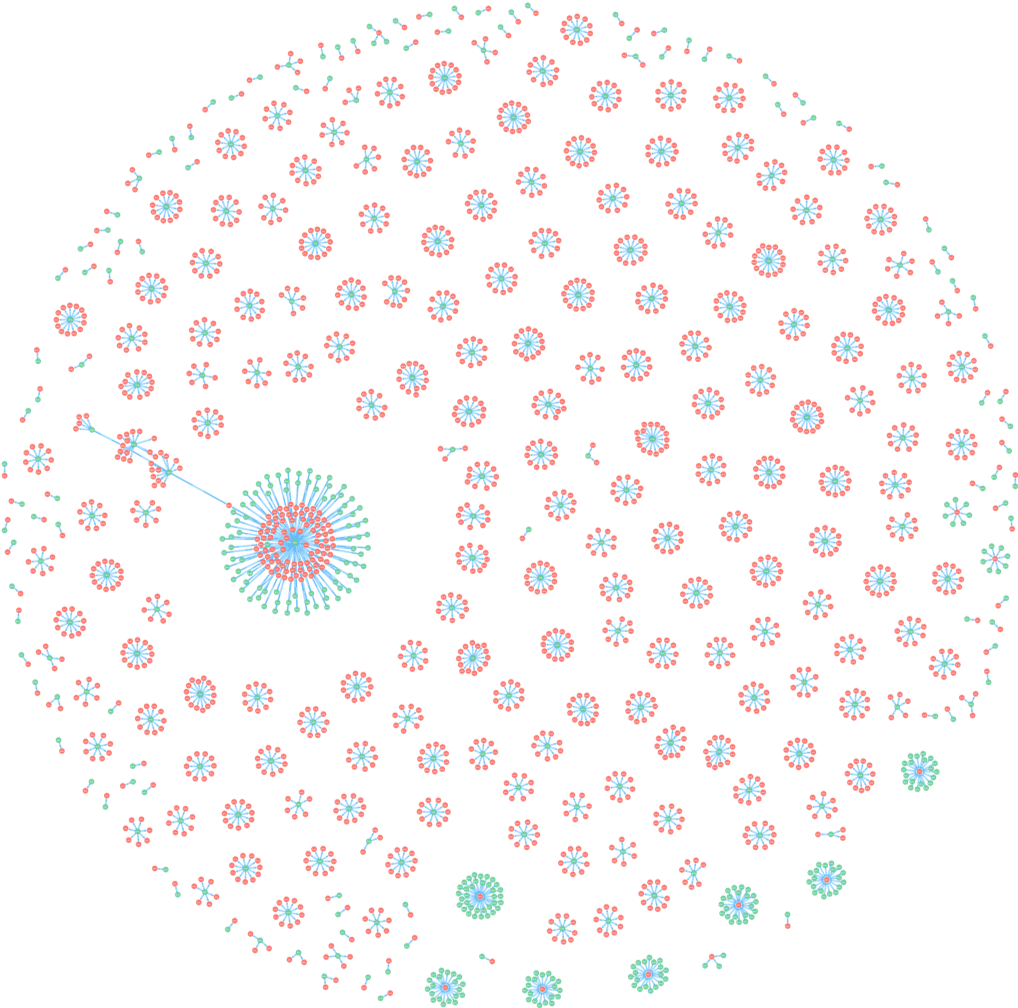
\includegraphics[scale=0.35]{graph-deathstar1.png}
    \caption{A network graph example featuring a subset of LANL source, user and host to destination, user and host.}
  \end{center}
  \label{figure:DeathStar1}
\end{figure}

%The figure above is a network graph of source, user and host to destination, user and host.

%%  HERE IS THE DEATHSTAR, SECOND OF TWO
\begin{figure}
  \centering
  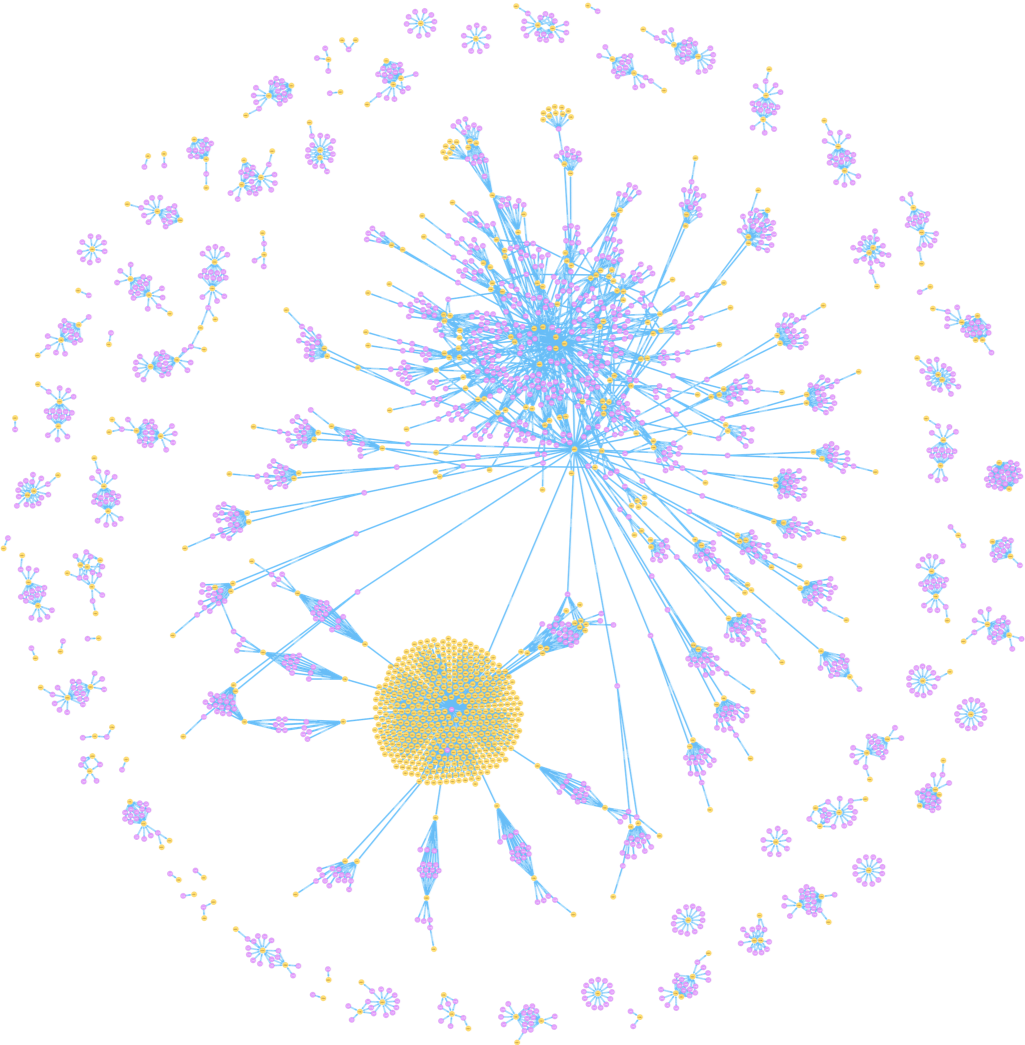
\includegraphics[scale=0.35]{graph-deathstar2.png}
  \caption{A network graph example featuring a subset of LANL source and destination user to source and destination host.}
  \label{figure:DeathStar2}
\end{figure}

%\begin{center}
%  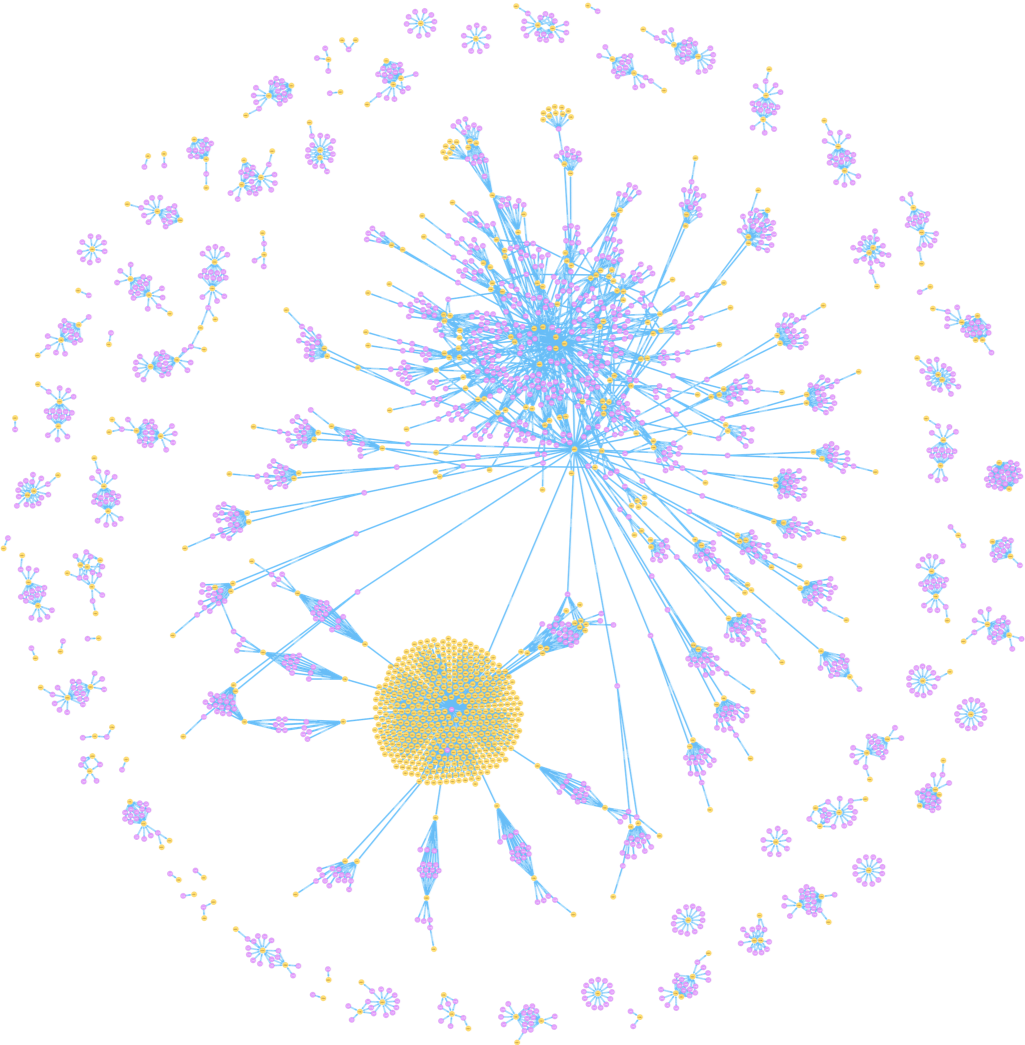
\includegraphics[scale=0.35]{graph-deathstar2.png}
%  \caption{Death star 2.}
%\end{center}

%The figure above is a network graph of source and destination user to source and destination host.

Features of interest include time, source user, destination user, source computer, and destination computer.  An \texttt{is\_malicious} feature indicates malicious red team data.  The raw dataset used for this research is structured as in \textbf{Table 1}. \textbf{Figure 1} shows a graph of network connections in which a source user-source computer (green node) connects to a destination user-destination computer (red node) along a blue edge.  \textbf{Figure 2}
is another graph depicting the relationship between users and computers: a source user-destination user (yellow node) connects to a source computer-destination computer (pink node) along a blue edge.
%We used \textbf{Figure 1} and \textbf{Figure 2} during our exploratory data analysis.

\begin{table*}[t]
  \centering
  \begin{tabular}{|c|c|c|c|c|c|c|}
  \hline
    & \texttt{time} & \texttt{src\_user} & \texttt{dest\_user} & \texttt{src\_comp} & \texttt{dest\_comp} & \texttt{is\_malicious} \\
  \hline
  0 & 1             & \texttt{U6@DOM1}   & \texttt{U6@DOM1}    & \texttt{C606}      & \texttt{C1065}      & 0                      \\
  \hline
  1 & 1             & \texttt{U6@DOM1}   & \texttt{U6@DOM1}    & \texttt{C606}      & \texttt{C529}       & 0                      \\
  \hline
  2 & 1             & \texttt{U6@DOM1}   & \texttt{U6@DOM1}    & \texttt{C606}      & \texttt{C529}       & 0                      \\
  \hline
  3 & 1             & \texttt{U14@DOM2}   & \texttt{U6@DOM1}    & \texttt{C616}      & \texttt{C29}       & 1                      \\
  \hline
  \end{tabular}
  \caption{Example of LANL source data.}
  \label{tab:1}
\end{table*}

\subsection{Probability Features}
The first features created were based on the frequency of a given condition.  Four features were created using this method.
%The frequencies were computed for various combinations of src\_user, dest\_user, src\_comp, and dest\_comp.
%The names of features created with this method are $\mathcal P(\texttt{dest\_user}|\texttt{src\_user})$, \\ $\mathcal P(\texttt{dest\_comp}|\texttt{src\_comp})$, $\mathcal P(\texttt{src\_comp}|\texttt{dest\_comp})$, and
%$\mathcal P(\texttt{dest\_comp}|\texttt{dest\_all\_user})$.  In order to create each of these features, a subset of the data is taken based on the conditional variable.  For instance, the first feature
%($\mathcal P(\texttt{dest\_user}|\texttt{src\_user})$) is created by first creating a set of all possible \texttt{src\_users} and all possible \texttt{dest\_users}.  Then, we loop through the set of \texttt{src\_users} and find the subset from
%!TEX encoding = UTF-8 Unicode the full data population where \texttt{src\_user} = SETsrc\_useri. Once we have the subset for a given \texttt{src\_user}, the frequency of each \texttt{dest\_user} is computed and stored in a dictionary to be %retrieved later.  This process is iterated for each of the four probability features declared in this section.  Once each dictionary is computed, the dictionaries are then used for translating each authentication record from the dataset into %probability features. Once this process is completed, the data fits the format indicated in Table 2.
%\begin{table*}[t]
%  \small
%  \scalebox{1.5}
%  \centering
%  \begin{tabular}{|c|c|c|c|}
%  \hline
%  $\mathcal P(\texttt{dest\_user|src\_user})$ & $\mathcal P(\texttt{dest\_comp|src\_comp})$ & $\mathcal P(\texttt{src\_comp|src\_user})$ & $\mathcal P(\texttt{dest\_comp|dest\_user})$ \\
%  \hline
%  0.962486                                    & 0.002706                                    & 1.0                                        & 0.028571                                     \\
%  \hline
%  0.962486                                    & 0.033559                                    & 1.0                                        & 0.171429                                     \\
%  \hline
%  0.962486                                    & 0.033559                                    & 1.0                                        & 0.171429                                     \\
%  \hline
%  0.962486                                    & 0.005954                                    & 1.0                                        & 0.042857                                     \\
%  \hline
%  0.962486                                    & 0.001624                                    & 1.0                                        & 0.028571                                     \\
%  \hline
%  \end{tabular}
%  \caption{Calculated features}
%  \label{tab:2}
%\end{table*}

We adopt the convention that if $\mathcal S$ is a (finite) set, then $n(\mathcal S)$ denotes the cardinality of $\mathcal S$, i.e., the count of distinct elements of $\mathcal S$.  Let $X$ denote the original set of data as indicated in \textbf{Table 1}, i.e. a two-dimensional array with columns \texttt{timestamp}, \texttt{src\_user}, \texttt{dest\_user}, \texttt{src\_comp}, \texttt{dest\_comp}, and \texttt{is\_malicious}.  For our purposes, it is necessary to think of $X$ as a set whose elements are the rows of the table;  so, using the cardinality notation, $n(X)$ indicates the number of rows in our table.  Let $\mathcal U$ and $\mathcal C$ denote the sets of all users and computers listed in our network data.  Define
distinguished subsets $\mathcal{U_S}$ and $\mathcal{U_D}$ to be the set of all source users and destination users in our data;  likewise let $\mathcal{C_S}$ and $\mathcal{C_D}$ denote the sets of all source computers and destination computers.

Now, for a particular user $a$ in $\mathcal{U}$, let $XU_a$ denote the subset of $X$ where $a$ is listed as the source user, and let $XU^a$ denote the subset of $X$ where $a$ is listed as the destination user (think of these as a
selection of particular rows from $X$).  Similarly, for a particular computer $k$ in $\mathcal C$, let $XC_k$ denote the subset of $X$ where $k$ is listed as the source computer, and let $XC^k$ denote the subset of $X$ where $k$ is listed as the
destination computer.

Assuming that $a\in\mathcal{U_S}$, $b\in\mathcal{U_D}$, $k\in\mathcal{C_S}$, and $j\in\mathcal{C_D}$, we calculate the following conditional probabilities:
\begin{enumerate}
  \item The conditional probability that $b$ is the destination user, given that $a$ is the source user
  $$\mathcal P(XU^b|XU_a) = \frac{n(XU^b\cap XU_a)}{n(XU_a)},$$
  \item The conditional probability that $j$ is the destination computer, given that $k$ is the source computer
  $$\mathcal P(XC^j|XC_k) = \frac{n(XC^j\cap XC_k)}{n(XC_k)},$$
  \item The conditional probability that $k$ is the source computer, given that $a$ is the source user
  $$\mathcal P(XC_k|XU_a) = \frac{n(XC_k\cap XU_a)}{n(XU_a)},\textrm{ and}$$
  \item The conditional probability that $j$ is the destination computer, given that $b$ is the destination user.
  $$\mathcal P(XC^j|XU^b) = \frac{n(XC^j\cap XU^b)}{n(XU^b)}.$$
\end{enumerate}

These four conditional probabilities constitute engineered features used as input to the models as indicated in \textbf{Table 2}.

%
% du|su 
% dc|sc
% sc|su
% dc|du
%

\subsection{Hourly Metrics}
We partitioned our data into one hour bins for capturing sequences of events changing through time.  For each row of the table, find the quotient of the timestamp and 3600 (count of seconds in one-hour) and apply a ceiling function to round up to the next whole number.  In \textbf{Table 1}, the time column indicates the index of the hour in which the event took place.

We create the first of two features by counting how many distinct destination hosts to which a given source host has authenticated, and then grouped by each hour bin.  We then do the same for users by computing how many
destination users each source has use to authenticate, and then also grouped by each hour bin. After this process is completed, the final data is structured as indicated in \textbf{Table 2}.

\begin{table*}[t]
  \small	
  \centering
  \begin{tabular}{|c|c|c|c|c|c|c|}
  \hline
  $\mathcal P(\texttt{dest\_user|}$\hfill & $\mathcal P(\texttt{dest\_comp|}$\hfill & $\mathcal P(\texttt{src\_comp|}$\hfill & $\mathcal P(\texttt{dest\_comp|}$\hfill & \texttt{dc\_dest\_comp}\hfill  & \texttt{dc\_dest\_comp}\hfill & \texttt{is\_malicious} \\
              \hfill$\texttt{src\_user})$ &             \hfill$\texttt{src\_comp})$ &                \hfill$\texttt{src\_user})$ &                \hfill$\texttt{dest\_user})$ & \hfill\texttt{\_by\_src\_comp} &    \hfill\texttt{\_by\_src\_user} & \                      \\
  \hline
  0.96                                    & 0.0027                                      & 1.0                                        & 0.029                                       & 6                                  & 3                                 & 0                      \\
  \hline
  0.96                                    & 0.0336                                      & 1.0                                        & 0.171                                       & 6                                  & 3                                 & 0                      \\
  \hline
  0.96                                    & 0.0336                                      & 1.0                                        & 0.171                                       & 6                                  & 3                                 & 0                      \\
  \hline
  0.96                                    & 0.0060                                      & 1.0                                        & 0.043                                       & 6                                  & 3                                 & 0                      \\
  \hline
  0.96                                    & 0.0016                                      & 1.0                                        & 0.029                                       & 6                                  & 3                                 & 0                      \\
  \hline
  \end{tabular}
  \caption{Calculated features as input data for the autoencoder.}
  \label{tab:2}
\end{table*}

\begin{figure}
  \centering
  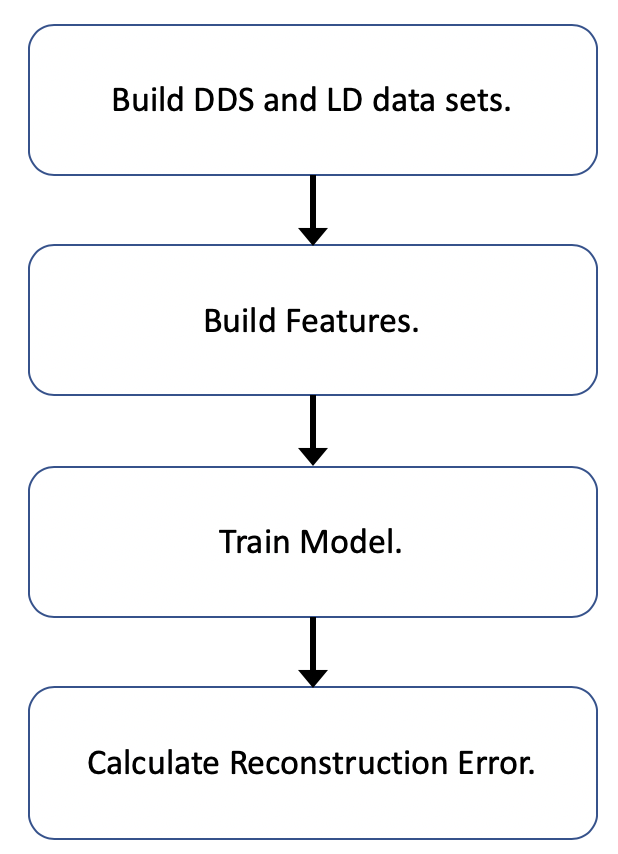
\includegraphics[scale=0.5]{Pipeline1.png}
  \caption{Data flow pipeline.}
  \label{figure:autoencoder}
\end{figure}

\section{Methods}

%\subsection{Description of Data Set created for analysis}

%The Los Alamos dataset was shrunk down to a 4 gigabyte file as described in section 2b. The dataset contains a timestamp, a source computer, and a destination computer. All of the events in the dataset
%were successful authentication events.  The other two datasets were untouched from their initial creation for our purposes.

%\subsection{Potential Data Science Approach}

%So far we are considering three approaches to this problem.

%Because cyber attacks are likely to include uncommon network connections, comparison of a network connection distribution over a short time span to a much larger block of connections establishing a pattern of normal traffic, a chi-square test is used to detect network abnormality during the short time span.

%Because a network cyber attack by necessity usually involves lateral movement, an attack is detectable by applying the very definition of lateral movement:  we hunt for all strings of network connections
%$A\rightarrow B\rightarrow C\rightarrow D\rightarrow\cdots$.  These are actual instances of lateral movement.

%We also will hunt for lateral movement by using an autoencoder neural network for anomaly detection. This represents an unsupervised approach to network activity classification. The idea came about due to the sophistication of the question. Several models were thought about in preliminary discussions including unsupervised clustering, SVM, and others. We think an autoencoder can improve detection of lateral movements if we transform network activity into a graph and feed into the autoencoder. This will lower the dimensions and pull out the most important features that the neural net will learn patterns off of over time.

\subsection{Autoencoders}

\textbf{Autoencoders} (AEs) have been proven to perform well in different types of anomaly detection problems. AE architecture and function is based on a classical unsupervised model called the encoder-decoder function
\cite{SAKURADA, AN, RANZATO}.  However, AEs can be considered to be semi-supervised learning due to the involvement of reconstruction error scoring \cite{AN}. 

The basic anatomy of an AE has an encoder function $f$ and a decoder function $g$. If $X$ represents input data, $Y = f(X)$ is the encoded data, and $Z = g(Y)$ is the decoded data. A well trained autoencoder should closely approximate the
identity function on the input data, i.e., the \textbf{reconstruction} $g(f(X))$ should be nearly the same as the original input data $X$.  The encoder will learn important features based on the input, but the reconstructed data will
not perfectly match the input. This helps the autoencoder to learn generalized mappings of the original features \cite{CHARTE,PEDREGOSA,KINGMA}. 

We developed four autoencoder models to evaluate in our research.  The first model was a \textit{vanilla} autoencoder (V-AE) consisting of only three layers and configured as 6-2-6;  the second model (D-AE) was a deeper version consisting of five layers 6-3-2-3-6;  the third model featured an asymmetric (or ``staggered'') encoder-decoder structure (S-DAE), layered 6-3-2-3-4-5-6;  finally, the fourth model used an architecture which was the reverse of the third, i.e., layered 6-5-4-3-2-3-6
(RS-DAE). 

We used Keras with TensorFlow to build and optimize our AE models utilizing Python.  We utilized a hybrid architecture of hyperbolic tangent ($\tanh$) activation layers and rectified linear unit (ReLU) activation layers \cite{CHOLLET}.  The first layer was regularized with an $\ell^1$ penalty of $10^{-5}$ for each model.  %Our model was compiled with the Adam optimizer and we used mean squared error (MSE) to calculate the loss \cite{KINGMA}.  We scaled our features with the MinMaxScaler() in ScikitLearn \cite{BENGIO,PEDREGOSA,CHOLLET}.  Cross-validation was used to calibrate and measure reproducibility by utilizing a 10-fold stratified shuffle of the input data.

\subsection{Technology Stack for Research}

\subsection{Model Preprocessing and Training}
We scaled our features with the \texttt{MinMaxScaler} function in Scikit-Learn \cite{BENGIO,PEDREGOSA,CHOLLET}. Our training and test data were split 90 / 10 using a random seed with the \texttt{Preprocessing} module from Scikit-Learn. Each model fit the training data over 5 epochs with a batch size of 1024. Our model was compiled with the Adam optimizer and we used mean squared error (MSE) to calculate the loss \cite{KINGMA}. We assessed our training by plotting the minimization of our objective function during training vs. epochs \cite{PEDREGOSA,CHOLLET} .

\subsection{Reconstruction Error}
%To evaluate our AE models as an unsupervised learner, we determined a function that could calculate a reconstruction based score.
We used mean squared error (MSE) to calculate the error.
%\begin{enumerate}
%  \item[]\textbf{INPUT:} Dataset $X$ including anomalous subset $A = \{x^{(i)}|i = 1, 2, \dots, N\}$;  Let $\alpha>0$ signify an error threshhold. 
%  \item[]\textbf{OUTPUT:}  reconstruction error $\|x - \hat x\|$
%  \item[]\quad $\phi, theta \longleftarrow$ train an autoencoder using the normal dataset $X$.
%\end{enumerate}
To do this, after training, we ran the \texttt{predict} function from our fitted models on our test data. The predictions were compared back to the test data as by our MSE scoring formula. In the case of our design, a high reconstruction error would indicate and be treated as an anomaly.  % (1, else 0).
To evaluate the reconstruction errors, we defined a manual threshold so that if any reconstructed value exceeded the set threshold it would be labeled as an anomaly. This threshold was manually optimized and set for all models.  Subsequently, we used our binary labeled array to calculate a confusion matrix as well as our other key metrics of interest. We also visually plotted out each MSE vs. data point index to visually assess the scoring. We repeated this processes throughout cross validation. 

%%  HERE IS THE GRAPHICAL DEPICTION OF OUR INEXPLICABLY ASYMMETRICAL AUTOENCODER
%\begin{figure}
%  \centering
%  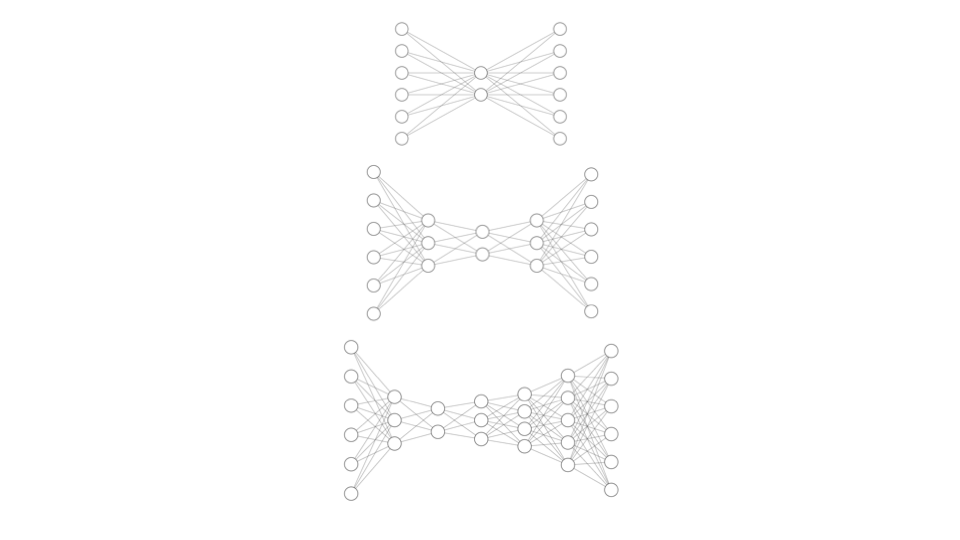
\includegraphics[scale=0.45]{AE_all_three.png}
%  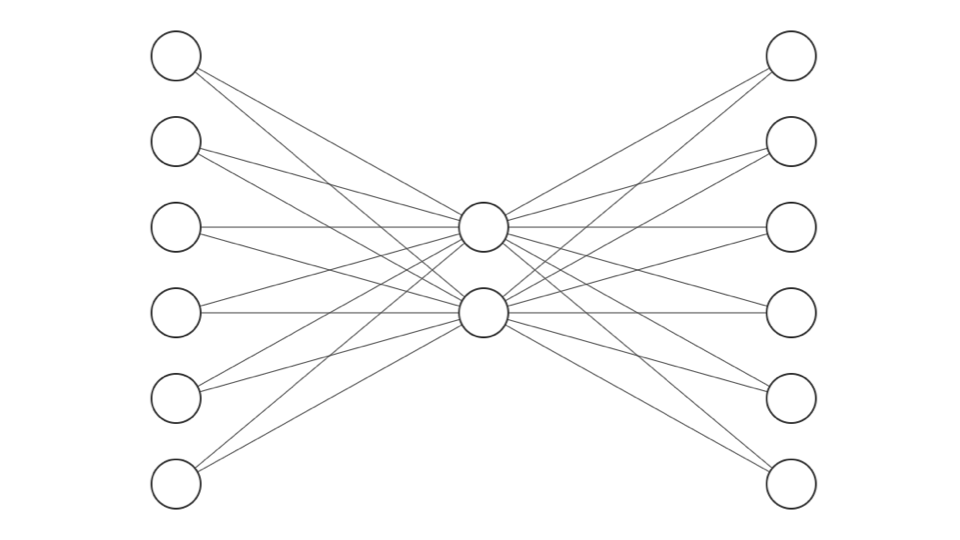
\includegraphics[scale=0.2]{AE6-2-6.png}
%  \caption{V-AE (6-2-6).}
%  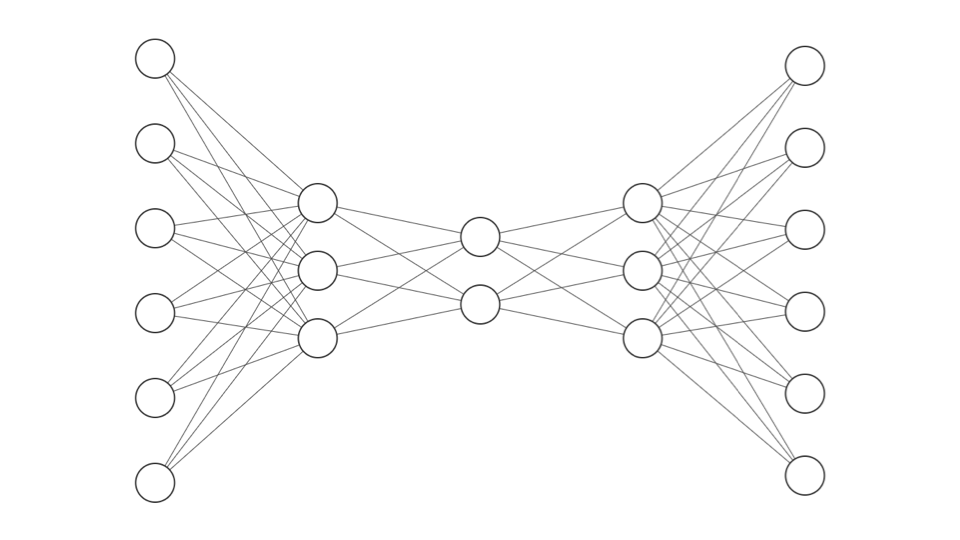
\includegraphics[scale=0.25]{AE6-3-2-3-6.png}
%  \caption{D-AE (6-3-2-3-6).}
%  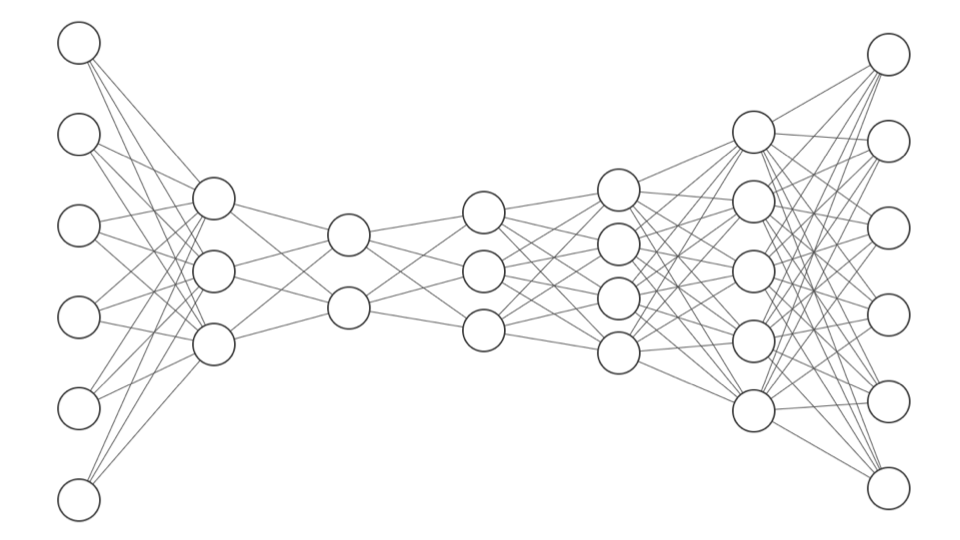
\includegraphics[scale=0.25]{AE6-3-2-3-4-5-6.png}
%  \caption{S-DAE (6-3-2-3-4-5-6).}
%  \label{figure:autoencoder}
%  \caption{The three autoencoders we tested.}
%\end{figure}

\begin{figure}[htbp]
\centering
\setlength{\lineskip}{\medskipamount}
\subcaptionbox{V-AE (6-2-6).\label{fig:1a}}{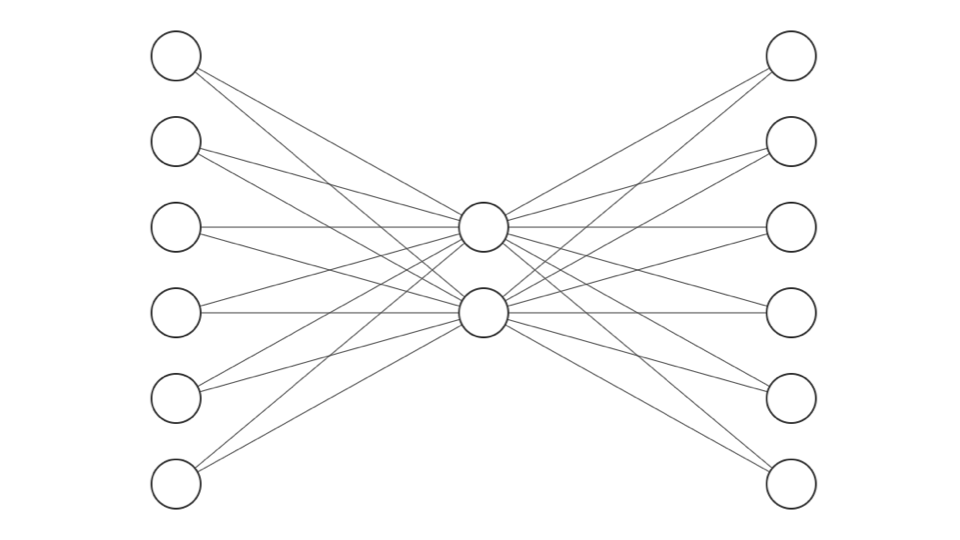
\includegraphics[scale=0.2]{AE6-2-6.png}}\hfill
\subcaptionbox{D-AE (6-3-2-3-6).\label{fig:1b}}{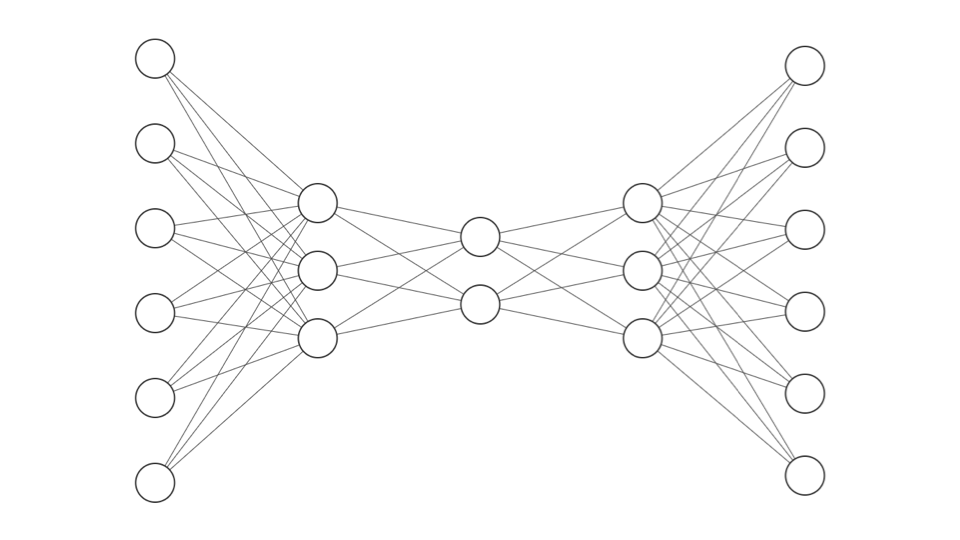
\includegraphics[scale=0.25]{AE6-3-2-3-6.png}}\hfill
\subcaptionbox{S-DAE (6-3-2-3-4-5-6).\label{fig:1c}}{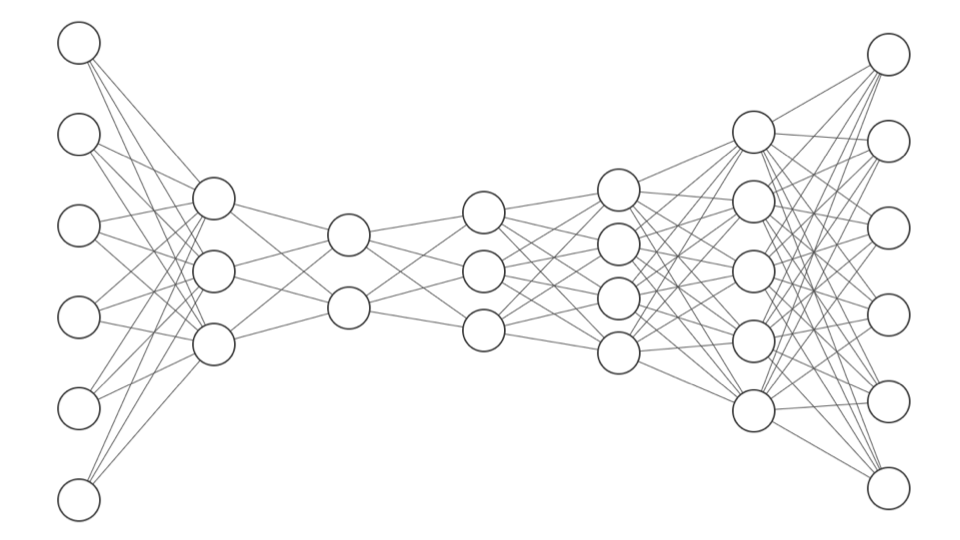
\includegraphics[scale=0.25]{AE6-3-2-3-4-5-6.png}}
\caption{The three autoencoders we tested.} \label{fig:1}
\end{figure}

%\section{Results}

%\subsection{Preliminary Results}

\begin{table}[t]
  \centering
  \begin{tabular}{|c|c|c|c|}
  \hline
  \textrm{Model}  & \textrm{FPR} & \textrm{Precision} & \textrm{Recall} \\
  \hline
  \textrm{V-AE}   & 0.0055       & 0.02               & 0.79            \\
  \hline
  \textrm{D-AE}   & 0.0085       & 0.03               & 0.81            \\
  \hline
  \textrm{S-DAE}  & 0.0095       & 0.03               & 0.81            \\
  \hline
  \textrm{RS-DAE} & 0.2038       & 0.00               & 0.00            \\
  \hline
%  \textrm{S-DAE (adjusted)} & 0. 994            & 0.04               & 0.81            \\
%  \hline
  \end{tabular}
  \caption{The preliminary analysis of the sub-sampled data set.}
  \label{tab:3}
\end{table}

\section{Results}

From the analysis, we conducted a stratified 10-fold cross-validation for the models on a developmental data set using \texttt{model selection} from Scikit-Learn.  Based on that, we assembled an aggregate confusion matrix, and analyzed several metrics including the recall, false positive rate, precision and accuracy.  We calculated the above metrics with the \texttt{classification report} and \texttt{confusion matrix} functions of Scikit-Learn \cite{PEDREGOSA}. 

%For the models, the precision ranged from 0.02 to 0.03, the recall ranged from 0.79 to 0.81, and the false positive rate ranged from 0.0055 to 0.0095.  
In the preliminary results, listed in \textbf{Table 3}, all AE models performed well except for RS-DAE, which had a high false positive rate.  Although the accuracy of RS-DAE was 0.99, the recall, precision, and fall-out were zero. Consequently, we rejected this model for its poor performance on the developmental data. The architecture of the remaining models can be seen in \textbf{Figure 4}. However, the V-AE, D-AE, and S-DAE performed with high accuracy and a false positive rate of 0.0055, 0.0085, and 0.0096 respectively. The respective recall values were 0.79, 0.81, and 0.81.% Although our precision was low, based on the other metrics we considered our preliminary results to outperform or comparable to other autonomous detection methods conducted on the LANL dataset \cite{HEARD2, BOHARA}. 


We moved on to evaluate our models on the larger dataset in which the same metrics were calculated under the same cross validation design. We found that our models improved in false positive rate and recall, but the change in precision remained negligible. The V-AE achieved a false positive rate of 0.0004 and a recall of 0.92. The D-AE and the S-DAE obtained a false positive rate of 0.0002. However, the S-DAE recall was slightly higher at 0.94 as compared to 0.93 from the D-AE model. When we used larger data set LD we saw that our autoencoders' false positive rate and recall not only maintained performance, but increased overall. These results are depicted in \textbf{Figure 5}.  Although our precision was low, based on the other metrics, we considered our results to meet or exceed the performance of other autonomous detection methods conducted on the LANL dataset \cite{HEARD2, BOHARA}. 

%Although we would ultimately expect an unsupervised method to increase productivity (i.e., decreasing time to detection), we did not have the ability to evaluate time as a metric during this research. 

\section{Related Work}
Unsupervised machine learning has been used to detect insider threats using deep and recurrent neural networks \cite{TUOR}.  Machine learning has also been used to detect attacks on web applications \cite{CHORAS}.

Other research has been conducted on the LANL dataset for anomaly detection protocols. A rule based visualization pattern discovery tool, APT-Hunter, conducted an experiment with a false positive rate of 0.00005 (0.005\%). Their model performed better than our AE models.  However, this platform required an analyst to manually look through patterns to identify potential threats, and was not automated to detect malicious events \cite{SIADATI}.  Another statistical approach devised by Heard et al. was used on the
LANL dataset to determine anomalies based on source computers only \cite{HEARD}.  More recently Sanders et al. \cite{BOHARA} provided a methodology using unsupervised ensemble approaches. Sanders et al. reached an overall average true positive
rate of detection of 0.89 with varying ranges of false positive rate performance. We have seen other unsupervised approaches in Chapter 9 of \textit{Data Science for Cyber-Security} relative to classifying red team events based on various spectral and normalized Laplacian embedding techniques on the LANL dataset \cite{HEARD2}.
%involving several spectral and normalized Laplacian embedding techniques \cite{HEARD2}.

Overall, to the best of our knowledge, we have not seen published identical approaches in which an AE was used specifically for detecting malicious events in the LANL dataset. 

%Next we ran the validation on the larger data set (see Figure 5).  Here, precision ranged from 0.003 to 0.005, the recall ranged from 0.92 to 0.93, and the false positive rate (FPR) improved to a range of 0.0002 to 0.0004.  We found that when training on the larger data set the FPR and recall improved markedly, while the precision dropped.  Based on the ten-fold validation, the deep and the staggered deep autoencoders exhibited the best performance.

\begin{figure}[htbp]
\centering
\setlength{\lineskip}{\medskipamount}
\subcaptionbox{False positive rates.\label{fig:1a}}{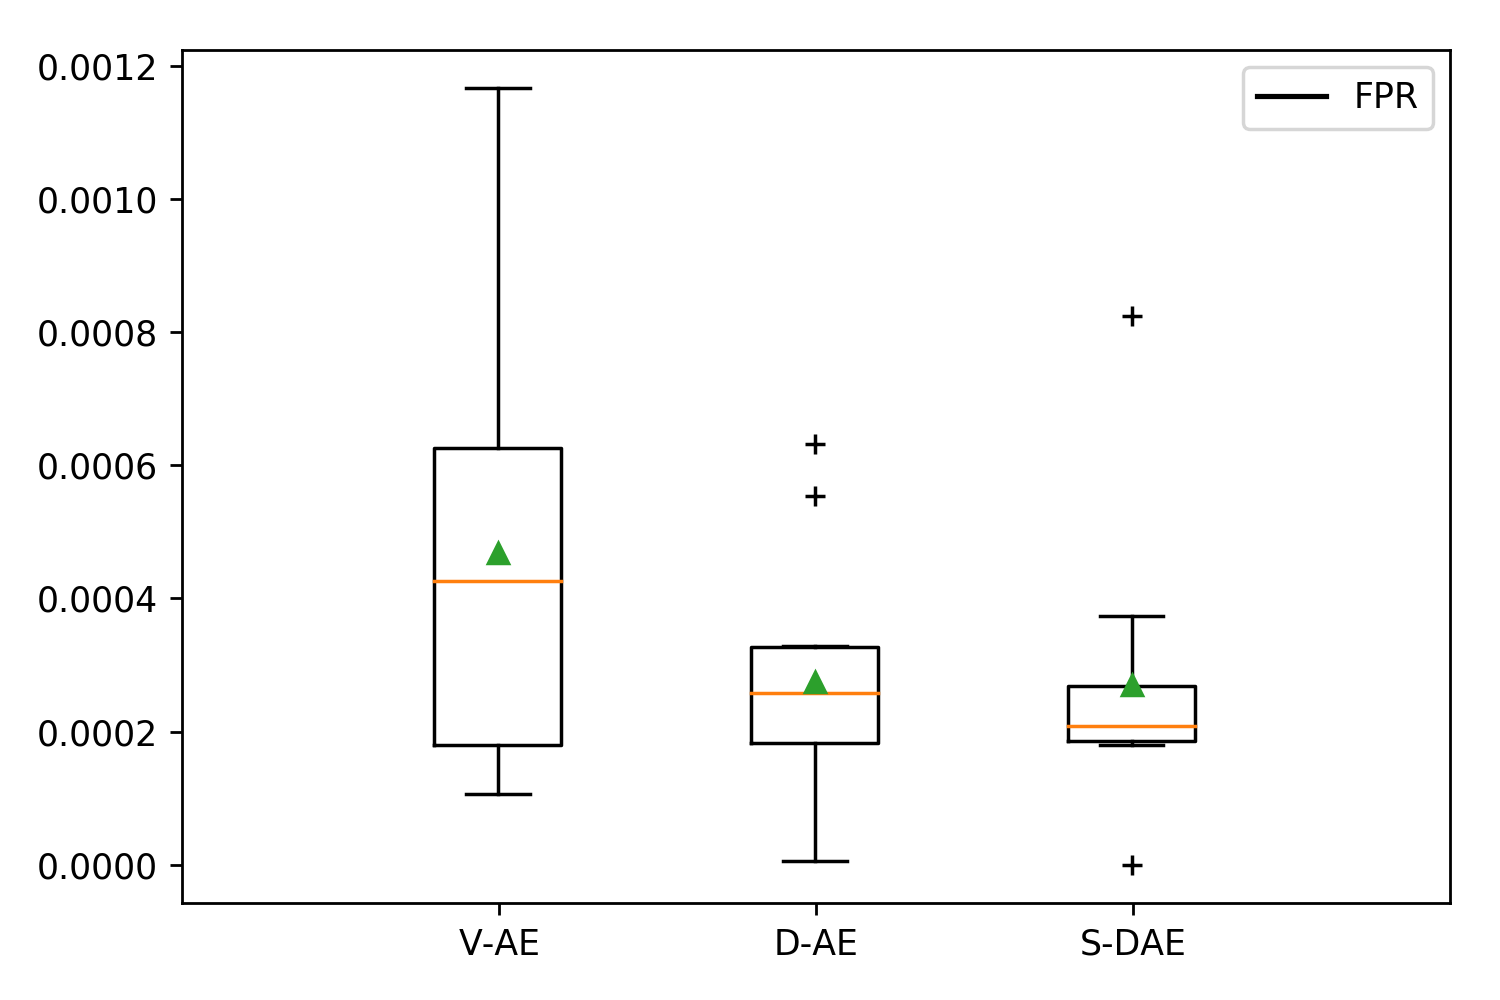
\includegraphics[scale=0.45]{FPR_test_big.png}}\hfill
\subcaptionbox{True positive rates.\label{fig:1b}}{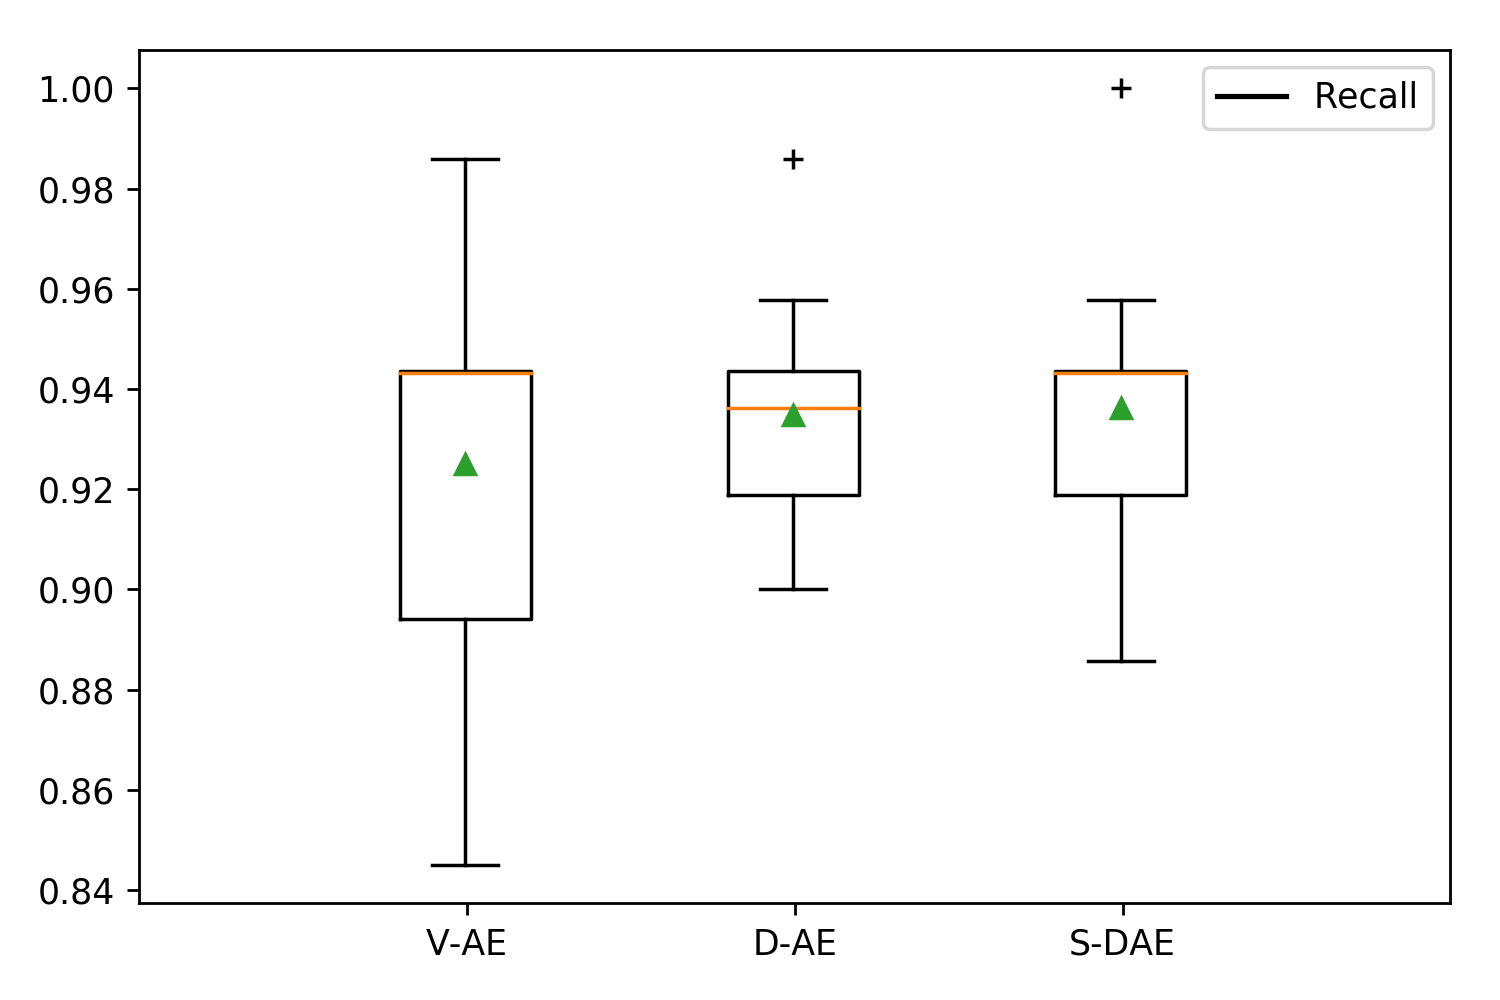
\includegraphics[scale=0.45]{Recall_test_big.png}}\hfill
\subcaptionbox{Calculated precision.\label{fig:1c}}{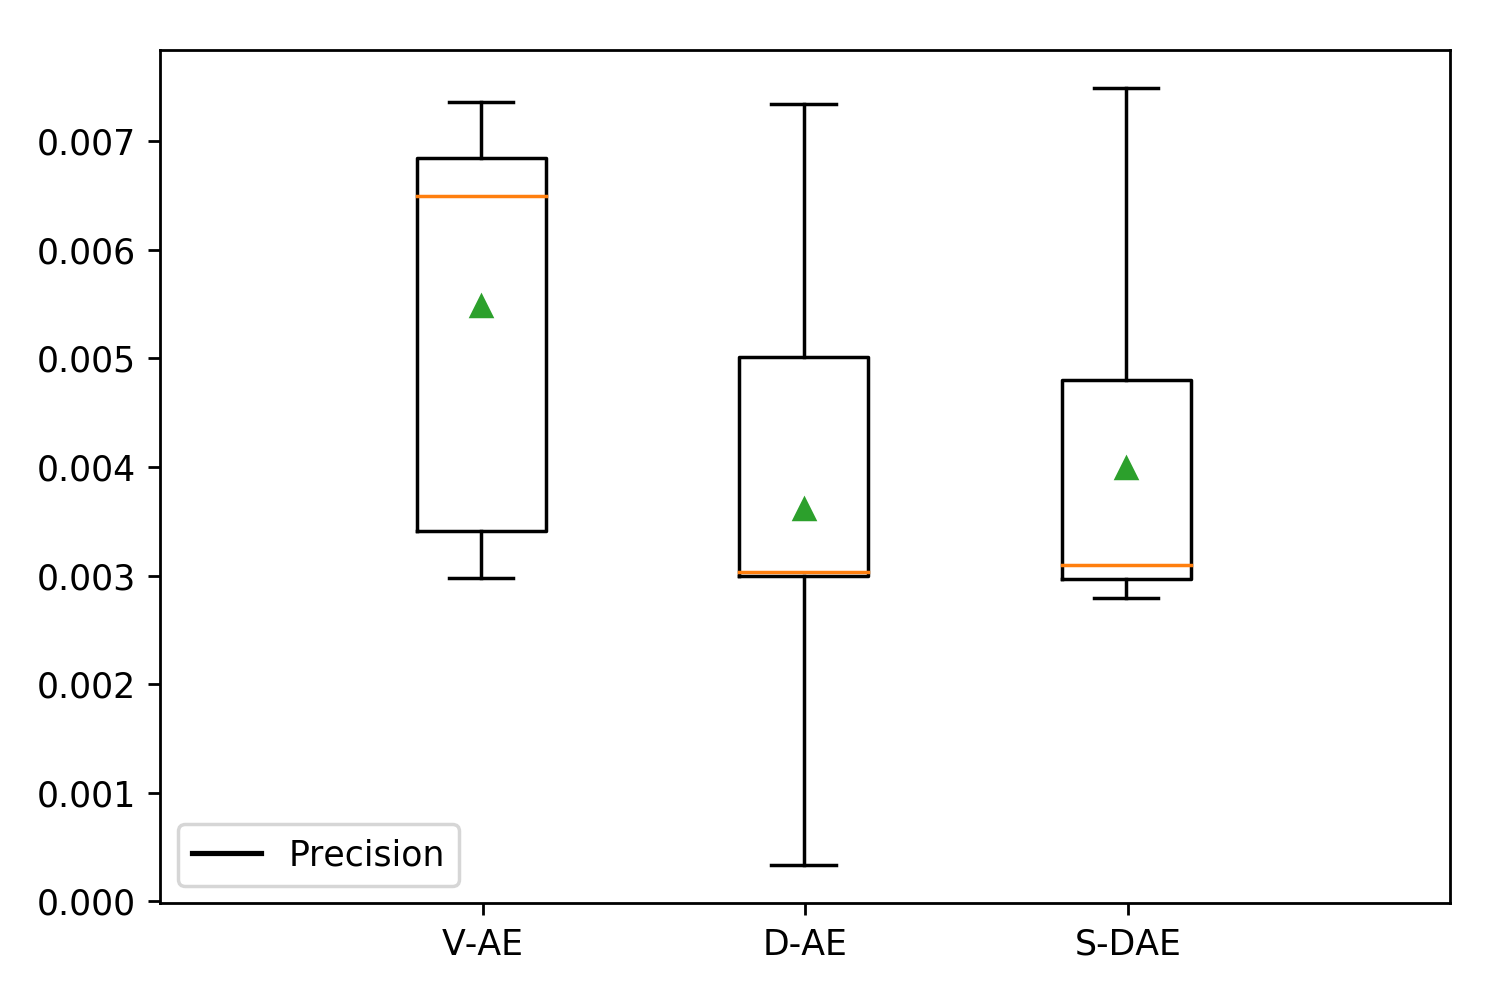
\includegraphics[scale=0.45]{Precision_test_big.png}}
\caption{Performance results for our three models.} \label{fig:1}
\end{figure}

%\begin{figure}
%  \centering
%  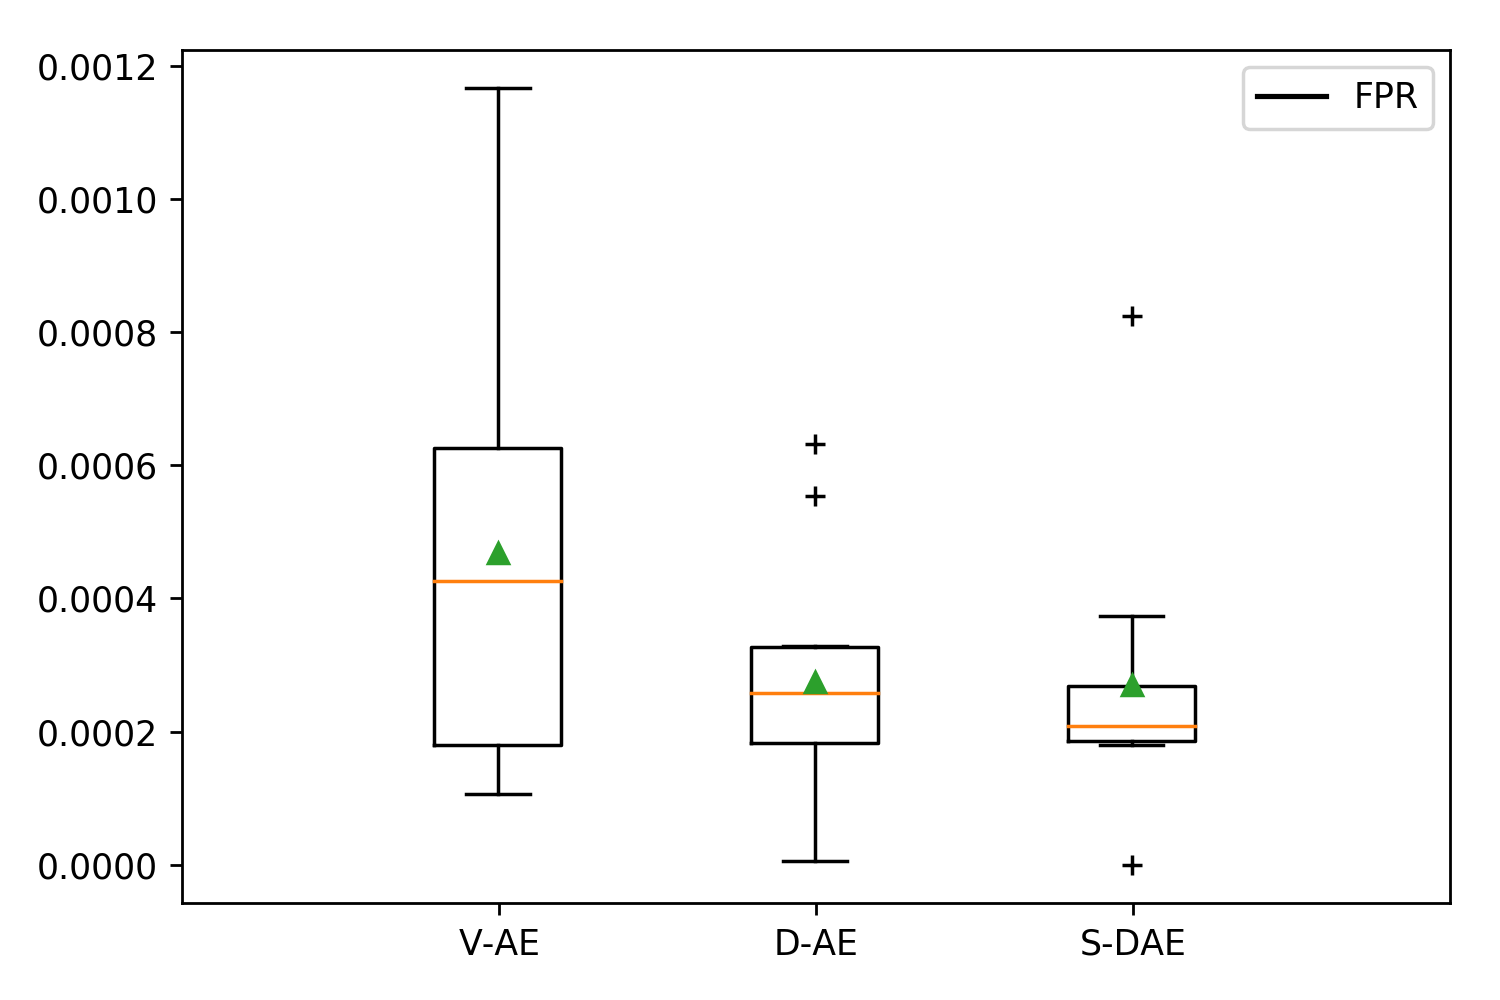
\includegraphics[scale=0.5]{FPR_test_big.png}
%  \caption{\small The false positive rate for the three models.}
%  \label{figure:autoencoder}
%\end{figure}
%\begin{figure}
%  \centering
%  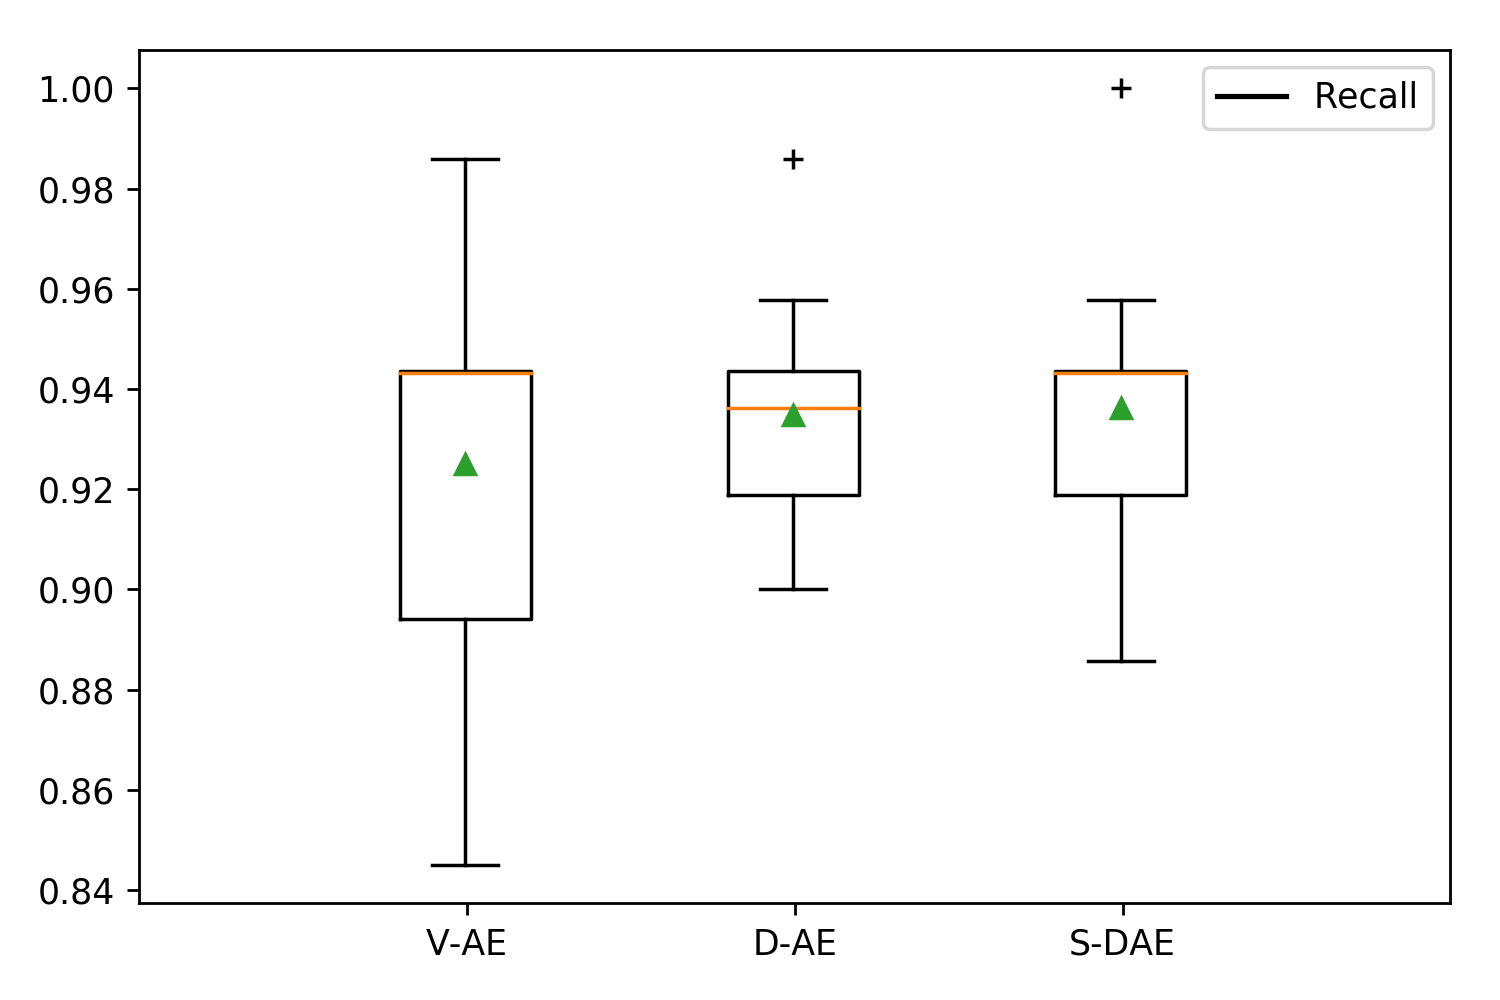
\includegraphics[scale=0.5]{Recall_test_big.png}
%  \caption{\small The true positive rate for the three models.}
%  \label{figure:autoencoder}
%\end{figure}
%\begin{figure}
%  \centering
%  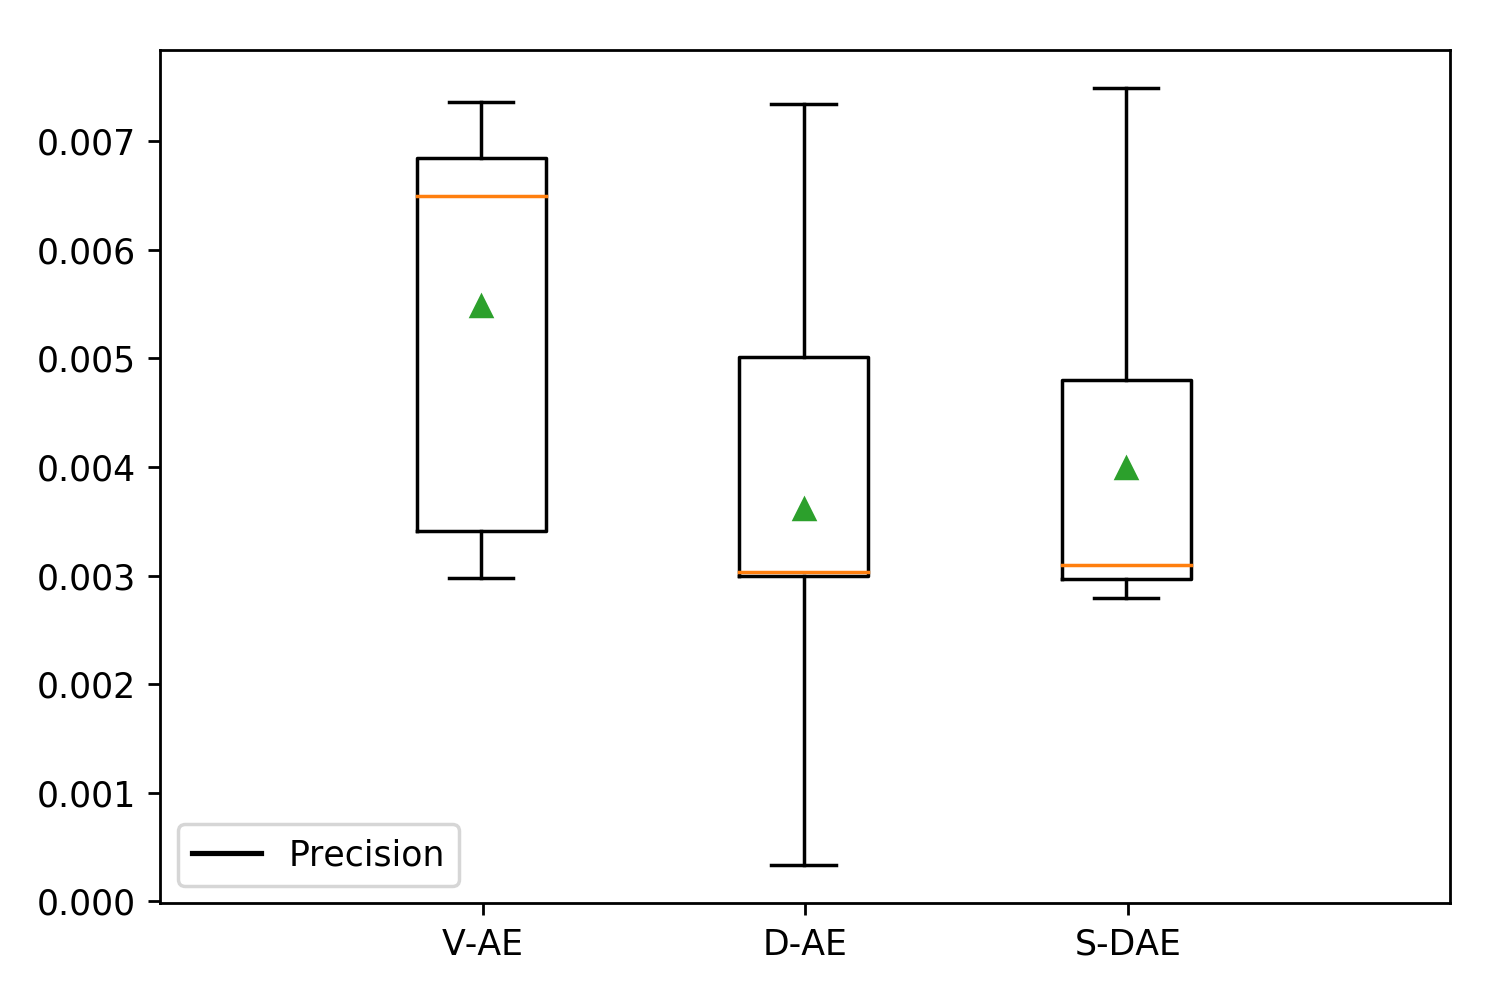
\includegraphics[scale=0.5]{Precision_test_big.png}
%  \caption{\small The precision for each of the three models.}
%  \label{figure:autoencoder}
%\end{figure}

%Other work has been conducted on this dataset for anomaly detection. A rule based visualization pattern discovery tool, APT-Hunter, conducted an experiment with the Los Alamos dataset with a 0.005\% false positive rate.
%However, this platform required analyst to manually look through patterns to identify potential threats, and was not automated to detect malicious events [1].  Another statistical approach devised by Heard et al. was used on
%the Los Alamos dataset in nature and sought to determine anomalies based on source computers only [2]. More recently Sanders et al. [3] provided a methodology using unsupervised ensemble approaches. They reached an
%overall an accuracy of detection of 88.7\% with varying ranges of false positive rate performance. Chapter 9 of Data Science for Cyber-Security has a chapter dedicated to classifying red team events that discussed embedding
%techniques on the LANL dataset involving several spectral and normalized Laplacian embedding techniques [4]. 

%\begin{table}[t]
%  \centering
%  \begin{tabular}{|l|r|r|}
%  \hline
%                    & \texttt{True} & \texttt{False} \\
%  \hline
%  \texttt{Positive} & 556930.3      & 5556.6         \\
%  \hline
%  \texttt{Negative} & 10.9          & 59.6           \\
%  \hline
%  \end{tabular}
%  \caption{Aggregate confusion matrix}
%  \label{tab:3}
%\end{table}

\section{Limitations and Future Work}

Several determining factors restricted our team in this study.
\begin{enumerate}
  \item \textit{Resources}: Our challenges to manage, manipulate, and train our model on the original LANL dataset was limited by our computational resources. We did utilize GPUs for the bulk of this work,
  however, testing preliminary ideas and experimentation on-the-fly was only feasible with smaller datasets. Having more dedicated computing power would have greatly helped our experimentation.
  \item \textit{Data Selection}: Our dataset was formulated to encompass data that would mimic a theoretical anomaly detection schema. We used all red team events as our base data and then selected all source
  and destination communications from within this subset from the overall dataset. To allow for noise that would be seen in a real-world system, we added additional selection of non-red team source hosts which
  may cause some underlying bias in our model; however, we believe that fundamentally our technique is validated. Re-evaluating the results on the full data set as well as exploring real-time solutions with
  this model would be an improvement. 
  \item \textit{Algorithm Design}: Choosing only a few models to evaluate has limited us in our protocol. In future work, we want to explore deeper and more complex architecture as a solution. We also believe
  that ensemble methods would be valuable to evaluate against our models. 
%%  \item We could have handled time data differently, and probably would be well motivated to do so if we were developing real-time cybercrime detection software${}^*$.
\end{enumerate}

% \section{Potential Challenges}
% The data transformation that will be used to feed into the autoencoder will have to be manually programmed. This part appears to be relatively novel as far as being used in association with an
% autoencoding neural network. We will have to spend a fair amount of time validating the transformation of data.

% Another challenge will be evaluation of the autoencoder. Since this is an unsupervised approach, we will have to consider advanced methods of evaluation such as cross validation techniques, understanding
% signal recognition, and loss calculations. 

\section{Discussion}
Anomaly detection for lateral movement is not new to the industry. Multiple methods, traditional and non-traditional, have been available with varying degrees of application.  %.. Talk about Traditional vs Non-Traditional ...
Some of the traditional signature-based tools, such as Snort, yield too many false positives, and so would flood analysts with alert messages such as `\texttt{ET POLICY PSexec service created}', when system administrators perform these actions
regularly \cite{CYRUS}. An analyst would exempt these system administrators' hosts from this specific detection leading to a potential blind spot for attackers to utilize.  Outside of traditional signature-based approaches addressing this issue, there have been other research in cybersecurity for detecting lateral movement using graphs. For instance, Sqrrl suggests detecting this traffic by learning common login patterns for users and ranking every login according to its anomalous nature\cite{SQRRL}.  In addition, there have been successful approaches using game theory and solving for saddle point strategies enabling the researchers to successfully detect the lateral movement and respond immediately by blocking the attacker \cite{FAWAZ}.

Autonomous cyber breach detection holds the promise of utility in a real-time system.  Network administrators would find it advantageous to be alerted of a cyber attack while it is underway as opposed to hours, days or months later.  Moreover, the paucity of verified network data
containing known cyber attacks suitable for training supervised algorithms leaves autonomous systems as a favorable option.  Such an approach applies to the more general problem of detecting unanticipated cyber attacker techniqes than traditional tools which seek to detect a particular kind of attack.

Autoencoders presently enjoy widespread application in the general area of anomaly detection.  They provide a robust method for learning generalized associations inside a dataset, in an unsupervised format\cite{AN,SAKURADA}.  We built and evaluated multiple autoencoders and tested them on the LANL dataset
to determine their effectiveness in detecting anomalous network activity.  We found that suitably structured autoencoders generally performed well on network authentication data.  We also discovered that increasing the dimension of the decoder improved several measures of the autoencoder's efficacy.  Additional research is needed.

%\section{Related Work}

%Others in the field have been motivated to look at related issues.  Unsupervised deep learning has been used to detect insider threats using deep and recurrent neural networks \cite{TUOR}.  Machine learning has
%also been used to detect attacks on web applications \cite{CHORAS}.
%%[insert relevant Cyber literature, Stoney/Alex?]

%Other work has been conducted on the LANL dataset for anomaly detection protocols. A rule based visualization pattern discovery tool, APT-Hunter, conducted an experiment with a false positive rate of 0.00005.
%However, this platform required analyst to manually look through patterns to identify potential threats, and was not automated to detect malicious events \cite{SIADATI}.  Another statistical approach devised by Heard et al. was used on the
%LANL dataset to determine anomalies based on source computers only \cite{HEARD}.  More recently Sanders et al. \cite{BOHARA} provided a methodology using unsupervised ensemble approaches. Sanders et al. reached an overall an accuracy
%of detection of 0.887 with varying ranges of false positive rate performance. Chapter 9 of Data Science for Cyber-Security has a chapter dedicated to classifying red team events that discussed embedding techniques on the LANL dataset
%involving several spectral and normalized Laplacian embedding techniques \cite{HEARD2}.

%Overall, to the best of our knowledge, we have not seen published identical approaches in which an AE was used specifically for detecting malicious events in the LANL dataset. 

\section{Conclusion}
Utilizing autoencoders for anomaly detection in authentication data has the potential to improve and automate parts of cybersecurity. We have demonstrated an autoencoder application, using a real-world use case for detecting anomalies, enabling increased productivity, preventing loss, and serving as a mechanism to detect lateral movement and other malicious events prematurely. 

% Detecting lateral movement is an essential aspect for all network defenders to detect as many attackers utilize legitimate tools that will not trip off any existing signature based detections after the attacker gains initial access.
% A chi square approach proved to produce a significant p-value for detecting this type of activity. In addition to this approach, the authors would also like to utilize multiple unsupervised machine learning techniques. One of the
% main approaches the authors have discussed would be to use a neural network autoencoder. Other future work would be to utilize clustering techniques or a support vector machine algorithm for anomaly detection. More work is expected
% to be performed to suggest multiple ways the security community and network defenders can detect lateral movement. 

\section{Acknowledgements}
We would like to express our gratitude to Professor Todd Gary of Lipscomb University for suggesting this direction for our research.  Thanks also to prof. Qingguo Wang for his advice to us for this research.
  
 %%$$\left[\begin{array}{rr} 556930.3 & 5556.6 \\ 10.9 & 59.6 \end{array}\right]$$

%  \begin{center}
%  \setlength{\unitlength}{1cm}
%  \begin{picture}(8, 7)
%  \thicklines
%  \put(1, 6){\circle{0.75}}
%  \put(1, 5){\circle{0.75}}
%  \put(1, 4){\circle{0.75}}
%  \put(1, 3){\circle{0.75}}
%  \put(1, 2){\circle{0.75}}
%  \put(1, 1){\circle{0.75}}
  
%  \put(2, 5.25){\circle{0.75}}
%  \put(2, 3.5){\circle{0.75}}
%  \put(2, 1.75){\circle{0.75}}
  
%  \put(3, 4.5){\circle{0.75}}
%  \put(3, 2.5){\circle{0.75}}
  
%  \put(4, 5.25){\circle{0.75}}
%  \put(4, 3.5){\circle{0.75}}
%  \put(4, 1.75){\circle{0.75}}
  
%  \put(5, 5.5){\circle{0.75}}
%  \put(5, 4.25){\circle{0.75}}
%  \put(5, 2.75){\circle{0.75}}
%  \put(5, 1.5){\circle{0.75}}

%  \put(6, 5.75){\circle{0.75}}
%  \put(6, 4.625){\circle{0.75}}
%  \put(6, 3.5){\circle{0.75}}
%  \put(6, 2.375){\circle{0.75}}
%  \put(6, 1.25){\circle{0.75}}

%  \put(7, 6){\circle{0.75}}
%  \put(7, 5){\circle{0.75}}
%  \put(7, 4){\circle{0.75}}
%  \put(7, 3){\circle{0.75}}
%  \put(7, 2){\circle{0.75}}
%  \put(7, 1){\circle{0.75}}

%  \thinlines
%  \put(1.275, 5.75){\vector(4, -3){.4}}
%  \put(1.3, 3.85){\vector(2, -1){.4}}
%  \put(2.275, 5){\vector(4, -3){.4}}
%  \put(2.28, 3.75){\vector(1, 1){.49}}
%  \end{picture}
%  \end{center}
    
  %% 6 3 2 3 4 5 6 


%We would like to acknowledge David Vasil for his expert direction and data validation for lateral movement activity.  

%\bibliography{FinalPaperBibliography} 
%\bibliographystyle{ieeetr}

\begin{thebibliography}{9}

\bibitem{BUSINESS}  %%	1
\textit{Cyber Crime to Reach \$2 Trillion By 2019: What Can We Do?},
Jana Rooheart,
\url{https://www.business.com/articles/cyber-crime-to-reach-2-trillion-by-2019-what-can-we-do/},
Feb. 22, 2017.

\bibitem{CYBERCRIMES}  %%  2
Steve Morgan, editor-in-chief, \textit{Cybercrimes Magazine}
\url{https://cybersecurityventures.com/hackerpocalypse-cybercrime-report-2016/},
Oct. 16, 2017.

\bibitem{HERJ}  %%  3
Lewie Dunsworth, L., and Kapadia, K.,
The Herjavec Group,
\textit{The 2019 Healthcare Cybersecurity Report}
\url{https://www.herjavecgroup.com/wp-content/uploads/2018/11/Herjavec-Group-2019-Healthcare-Cybersecurity-Report.pdf}
2018.

\bibitem{FAWAZ}  %%  4
 Fawaz, A., Bohara, A., Cheh, C., \& Sanders, W. H. (n.d.),
 \textit{Lateral Movement Detection Using Distributed Data Fusion},
 Retrieved from,
 \url{https://www.perform.illinois.edu/Papers/USAN\_papers/16FAW02.pdf}.

\bibitem{SORIA}  %%  5
 Soria-Machado, M., Abolins, D., Boldea, C., \& Socha, K.,
 \textit{Detecting Lateral Movements in Windows Infrastructure},
 Retrieved from \url{http://cert.europa.eu/static/WhitePapers/}
 \texttt{CERT-EU\_SWP\_17-002\_Lateral\_Movements.pdf}
 2017, February 27.

\bibitem{L.M.}  %%  6
 L. M. (n.d.),
 \textit{The Cyber Kill Chain}, Retrieved from
 \url{https://www.lockheedmartin.com/us/what-we-do/aerospace-defense/cyber/cyber-kill-chain.html}.

\bibitem{M}  %%  7
 M. (n.d.),
 \textit{Lateral Movement},
 Retrieved from \url{https://attack.mitre.org/wiki/Lateral\_Movement}.

\bibitem{SHU}  %%  8
 Shu, X., Tian, K., Ciambrone, A., \& Yao, D.,
 \textit{Breaking the Target: An Analysis of Target Data Breach and Lessons Learned},
 Retrieved from \url{https://arxiv.org/pdf/1701.04940.pdf},
 2017.
 
\bibitem{ABE}  %%  9
 Abe, S.,
 \textit{Detecting Lateral Movement in APTs--Analysis Approach}
 \textit{on Windows Event Logs},
 \url{https://www.first.org/resources/papers/conf2016/FIRST-2016-105.pdf},
 June 17, 2016.

\bibitem{CYRUS}  %%  10
 Cyrus, R.,
 \textit{Detecting Malicious SMB Activity Using Bro. Retrieved from }\url{https://www.sans.org/reading-room/whitepapers/detection/detecting-malicious-smb-activity-bro-37472},
 December 13, 2016.

\bibitem{KENT}  %%  11
 Kent, A.D.,
 \textit{Comprehensive, Multi-Source Cybersecurity Events},
 Los Alamos National Laboratory,
 Retrieved from \url{http://dx.doi.org/10.17021/1179829},
 2015.

\bibitem{SAKURADA}  %%  12
M. Sakurada, T. Yairi,
\textit{Anomaly Detection Using Autoencoders with Non-linear Dimensionality Reduction},
ACM Press, 2014, pp. 4--11, \url{http://dx.doi.org/10.1145/ 2689746.2689747}. 

\bibitem{AN}  %%  13
Jinwon An and Sungzoon Cho.,
\textit{Variational Autoencoder based Anomaly Detection using Reconstruction Probability (Technical Report)},
pp.1--18, SNU Data Mining Center,
2015.

\bibitem{RANZATO}  %%  14
Marc Aurelio Ranzato, Y-Lan Boureau, Sumit Chopra, and Yann LeCun,
\textit{Proceedings of the Eleventh International Conference on Artificial Intelligence and Statistics, vol.2},
Proceedings of Machine Learning Research (Meila, M. and Shen, X., ed.), pp. 371--379,
\url{http://proceedings.mlr.press/v2/ranzato07a/ranzato07a.pdf},
21--24 March, 2007.

\bibitem{CHARTE}  %%  15
David Charte, Francisco Charte, Salvador Garc{\'{\i}}a, Mar{\'{\i}}a Jos{\'{e}} del Jes{\'{u}}s, and Francisco Herrera,
\textit{A Practical Tutorial on Autoencoders for Non-linear Feature Fusion: Taxonomy, Models, Software and Guidelines},
\url{http://arxiv.org/abs/1801.01586},
Mon, 13 Aug 2018.

\bibitem{PEDREGOSA}  %%  16
Pedregosa, F., Varoquaux, G., Gramfort, A., Michel, V., Thirion, B., Grisel, O., Blondel, M., Prettenhofer, P., Weiss, R., Dubourg, V., Vanderplas, J., Passos, A., Cournapeau, D., Brucher, M., Perrot, M., and Duchesnay, E.
\textit{Scikit-learn: Machine Learning in {P}ython, Journal of Machine Learning Research, Vol. 12, pp. 2825--2830}
2011.

\bibitem{KINGMA}  %%  17
Diederik P. Kingma and Jimmy Ba,
\textit{Adam: {A} Method for Stochastic Optimization, CoRR, Vol. abs/1412.6980, Mon, 13 Aug 2018},
\url{http://arxiv.org/abs/1412.6980},
2014.

\bibitem{CHOLLET} %%  18
Chollet, Fran\c{c}ois and others,
\textit{Keras},
\url{https://keras.io},
2015.

\bibitem{BENGIO}  %%  19
Yoshua Bengio, Aaron Courville, Ian Goodfellow,
\textit{Deep Learning},
MIT Press,
\url{https://www.deeplearningbook.org},
2016.

\bibitem{HEARD2}  %%  20
N. Heard, N. Adams, P. Rubin-Delanchy, and M. Turcotte,
\textit{Data Science for Cyber-Security},
WORLD SCIENTIFIC (EUROPE),
\url{https://www.worldscientific.com/doi/abs/10.1142/q0167}
2018.

\bibitem{BOHARA}  %%  21
A. Bohara, M. A. Noureddine, A. Fawaz and W. H. Sanders,
\textit{An Unsupervised Multi-Detector Approach for Identifying Malicious Lateral Movement}, 2017 IEEE 36th Symposium on Reliable Distributed Systems (SRDS), pp. 224-233,
Hong Kong, 2017.

\bibitem{TUOR}  %%  22
Aaron Tuor, Samuel Kaplan, Brian Hutchinson, Nicole Nichols, and Sean Robinson,
\textit{Deep Learning for Unsupervised Insider Threat Detection in Structured Cybersecurity Data Streams}
arXiv preprint arXiv:1710.00811
2017.

\bibitem{CHORAS}  %%  23
Michal Choras and Rafal Kozik,
\textit{Machine learning techniques applied to detect cyber attacks on web applications}
Logic Journal of the IGPL, Volume 23, Issue 1, 1 February 2015, Pages 45?56,
\url{https://doi.org/10.1093/jigpal/jzu038}
2014.

\bibitem{SIADATI}  %%  24
H. Siadati, B. Saket and N. Memon,
\textit{Detecting malicious logins in enterprise networks using visualization}, 2016 IEEE Symposium on Visualization for Cyber Security (VizSec), pp. 1--8.,
Baltimore, MD, 2016.

\bibitem{HEARD}  %%  25
N. Heard and P. Rubin-Delanchy,
\textit{Network-wide anomaly detection via the Dirichlet process}, 2016 IEEE Conference on Intelligence and Security Informatics (ISI), pp. 220-224,
Tucson, AZ, 2016.

\bibitem{SQRRL}  %%  26
Adam Fuchs (Sqrrl), Ryan Nolette (Sqrrl)
  \textit{Threat Hunting for Lateral Movement},
 Retrieved from \url{https://resources.sei.cmu.edu/asset\_files/Presentation/2018\_017\_001\_512070.pdf}.

%\bibitem{CHEN}  %%  27
% P.-Y. Chen, S. Choudhury, L. Rodriguez, A.  O. Hero, and I. Ray,
% \textit{Enterprise Cyber Resiliency Against Lateral Movement: A Graph Theoretic Approach},
% Retrieved from \url{https://drive.google.com/file/d/0BwD3Ql0nv5RWdEFKR21xNjZ0UWc/view},
% 2016.

%1 .H. Siadati, B. Saket and N. Memon, "Detecting malicious logins in enterprise networks using visualization," 2016 IEEE Symposium on Visualization for Cyber Security (VizSec), Baltimore, MD, 2016, pp. 1-8.?%doi: 10.1109/VIZSEC.2016.7739582?
%2. N. Heard and P. Rubin-Delanchy, "Network-wide anomaly detection via the Dirichlet process," 2016 IEEE Conference on Intelligence and Security Informatics (ISI), Tucson, AZ, 2016, pp. 220-224.?%doi: 10.1109/ISI.2016.7745478

%3. A. Bohara, M. A. Noureddine, A. Fawaz and W. H. Sanders, "An Unsupervised Multi-Detector Approach for Identifying Malicious Lateral Movement," 2017 IEEE 36th Symposium on Reliable Distributed Systems (SRDS), Hong Kong, 2017, pp. 224-233.?%doi: 10.1109/SRDS.2017.31?
%4. @book{doi:10.1142/q0167,
%author = {Heard, Nick and Adams, Niall and Rubin-Delanchy, Patrick and Turcotte, Melissa},
%title = {Data Science for Cyber-Security},
%publisher = {WORLD SCIENTIFIC (EUROPE)},
%year = {2018},
%doi = {10.1142/q0167},
%address = {},
%edition   = {},
%URL = {https://www.worldscientific.com/doi/abs/10.1142/q0167},
%eprint = {https://www.worldscientific.com/doi/pdf/10.1142/q0167}}

%6. 
%@article{DBLP:journals/corr/abs-1801-01586,
%  author    = {David Charte and
%               Francisco Charte and
%               Salvador Garc{\'{\i}}a and
%               Mar{\'{\i}}a Jos{\'{e}} del Jes{\'{u}}s and
%               Francisco Herrera},
%  title     = {A practical tutorial on autoencoders for nonlinear feature fusion:
%               Taxonomy, models, software and guidelines},
%  journal   = {CoRR},
%  volume    = {abs/1801.01586},
%  year      = {2018},
%  url       = {http://arxiv.org/abs/1801.01586},
%  archivePrefix = {arXiv},
%  eprint    = {1801.01586},
%  timestamp = {Mon, 13 Aug 2018 16:47:04 +0200},
%  biburl    = {https://dblp.org/rec/bib/journals/corr/abs-1801-01586}}
%7.
%@InProceedings{pmlr-v2-ranzato07a,
%  title = 	 {A Unified Energy-Based Framework for Unsupervised Learning},
%  author = 	 {Marc?Aurelio Ranzato and Y-Lan Boureau and Sumit Chopra and Yann LeCun},
%  booktitle = 	 {Proceedings of the Eleventh International Conference on Artificial Intelligence and Statistics},
%  pages = 	 {371--379},
%  year = 	 {2007},
%  editor = 	 {Marina Meila and Xiaotong Shen},
%  volume = 	 {2},
%  series = 	 {Proceedings of Machine Learning Research},
%  address = 	 {San Juan, Puerto Rico},
%  month = 	 {21--24 Mar},
%  publisher = 	 {PMLR},
%  pdf = 	 {http://proceedings.mlr.press/v2/ranzato07a/ranzato07a.pdf},
%  url = 	 {http://proceedings.mlr.press/v2/ranzato07a.html}}

%3.
%https://www.deeplearningbook.org/ @book{Goodfellow-et-al-2016,
%    title={Deep Learning},
%    author={Ian Goodfellow and Yoshua Bengio and Aaron Courville},
%    publisher={MIT Press},
%    note={\url{http://www.deeplearningbook.org}},
%    year={2016}
%}

%9. 
%@misc{chollet2015keras,
%  title={Keras},
%  author={Chollet, Fran\c{c}ois and others},
%  year={2015},
%  howpublished={\url{https://keras.io}},
%}

%4.
%@article{scikit-learn,
% title={Scikit-learn: Machine Learning in {P}ython},
% author={Pedregosa, F. and Varoquaux, G. and Gramfort, A. and Michel, V.
%         and Thirion, B. and Grisel, O. and Blondel, M. and Prettenhofer, P.
%         and Weiss, R. and Dubourg, V. and Vanderplas, J. and Passos, A. and
%         Cournapeau, D. and Brucher, M. and Perrot, M. and Duchesnay, E.},
% journal={Journal of Machine Learning Research},
% volume={12},
% pages={2825--2830},
% year={2011}
%}

%5. 
%@article{DBLP:journals/corr/KingmaB14,
%  author    = {Diederik P. Kingma and
%               Jimmy Ba},
%  title     = {Adam: {A} Method for Stochastic Optimization},
%  journal   = {CoRR},
%  volume    = {abs/1412.6980},
%  year      = {2014},
%  url       = {http://arxiv.org/abs/1412.6980},
%  archivePrefix = {arXiv},
%  eprint    = {1412.6980},
%  timestamp = {Mon, 13 Aug 2018 16:47:35 +0200},
%  biburl    = {https://dblp.org/rec/bib/journals/corr/KingmaB14},
%  bibsource = {dblp computer science bibliography, https://dblp.org}
%}


%1.
%https://www.deeplearningbook.org/ @book{Goodfellow-et-al-2016,
%    title={Deep Learning},
%    author={Ian Goodfellow and Yoshua Bengio and Aaron Courville},
%    publisher={MIT Press},
%   note={\url{http://www.deeplearningbook.org}},
%    year={2016}
%}
%2. 
%@misc{chollet2015keras,
%  title={Keras},
%  author={Chollet, Fran\c{c}ois and others},
%  year={2015},
%  howpublished={\url{https://keras.io}},
%}
%
%3.
%@article{scikit-learn,
% title={Scikit-learn: Machine Learning in {P}ython},
% author={Pedregosa, F. and Varoquaux, G. and Gramfort, A. and Michel, V.
%         and Thirion, B. and Grisel, O. and Blondel, M. and Prettenhofer, P.
%         and Weiss, R. and Dubourg, V. and Vanderplas, J. and Passos, A. and
%         Cournapeau, D. and Brucher, M. and Perrot, M. and Duchesnay, E.},
% journal={Journal of Machine Learning Research},
% volume={12},
% pages={2825--2830},
% year={2011}
%}
%
%4. 
%@article{DBLP:journals/corr/KingmaB14,
%  author    = {Diederik P. Kingma and
%               Jimmy Ba},
%  title     = {Adam: {A} Method for Stochastic Optimization},
%  journal   = {CoRR},
%  volume    = {abs/1412.6980},
%  year      = {2014},
%  url       = {http://arxiv.org/abs/1412.6980},
%  archivePrefix = {arXiv},
%  eprint    = {1412.6980},
%  timestamp = {Mon, 13 Aug 2018 16:47:35 +0200},
%  biburl    = {https://dblp.org/rec/bib/journals/corr/KingmaB14},
%  bibsource = {dblp computer science bibliography, https://dblp.org}
%}


%\bibitem{lamport94}
%  Leslie Lamport,
%  \textit{\LaTeX: a document preparation system},
%  Addison Wesley, Massachusetts,
%  2nd edition,
%  1994.

\end{thebibliography}

\end{document}  